\chapter{Clustering}

Unsupervised Learning tasks differ from Supervised Learning tasks because the dataset contains no labels $y$: we cannot supervise the learning by comparing the predictions with a ground truth. Clustering is the most famous Unsupervised Learning task. A \textbf{cluster} is a group of data points that are close to each other, hence the goal of clustering is to detect groups of similar data points that are, in some sense, homogeneous.

Clustering can be used for image segmentation, as a pre-processing step and also to detect outliers. In networking it is used, for instance, to:
\begin{itemize}
    \item group traffic flows with similar behaviour (packet sizes, durations, rates) and discover the applications that generate them, without labelling a single flow;
    \item group hosts with similar traffic profiles, e.g. servers, workstations, IoT devices;
    \item detect anomalies: a flow or a host that does not fit any group deserves a closer look;
    \item compress measurements, by replacing each data point with the representative of its cluster.
\end{itemize}

\begin{figure}[h]
    \centering
    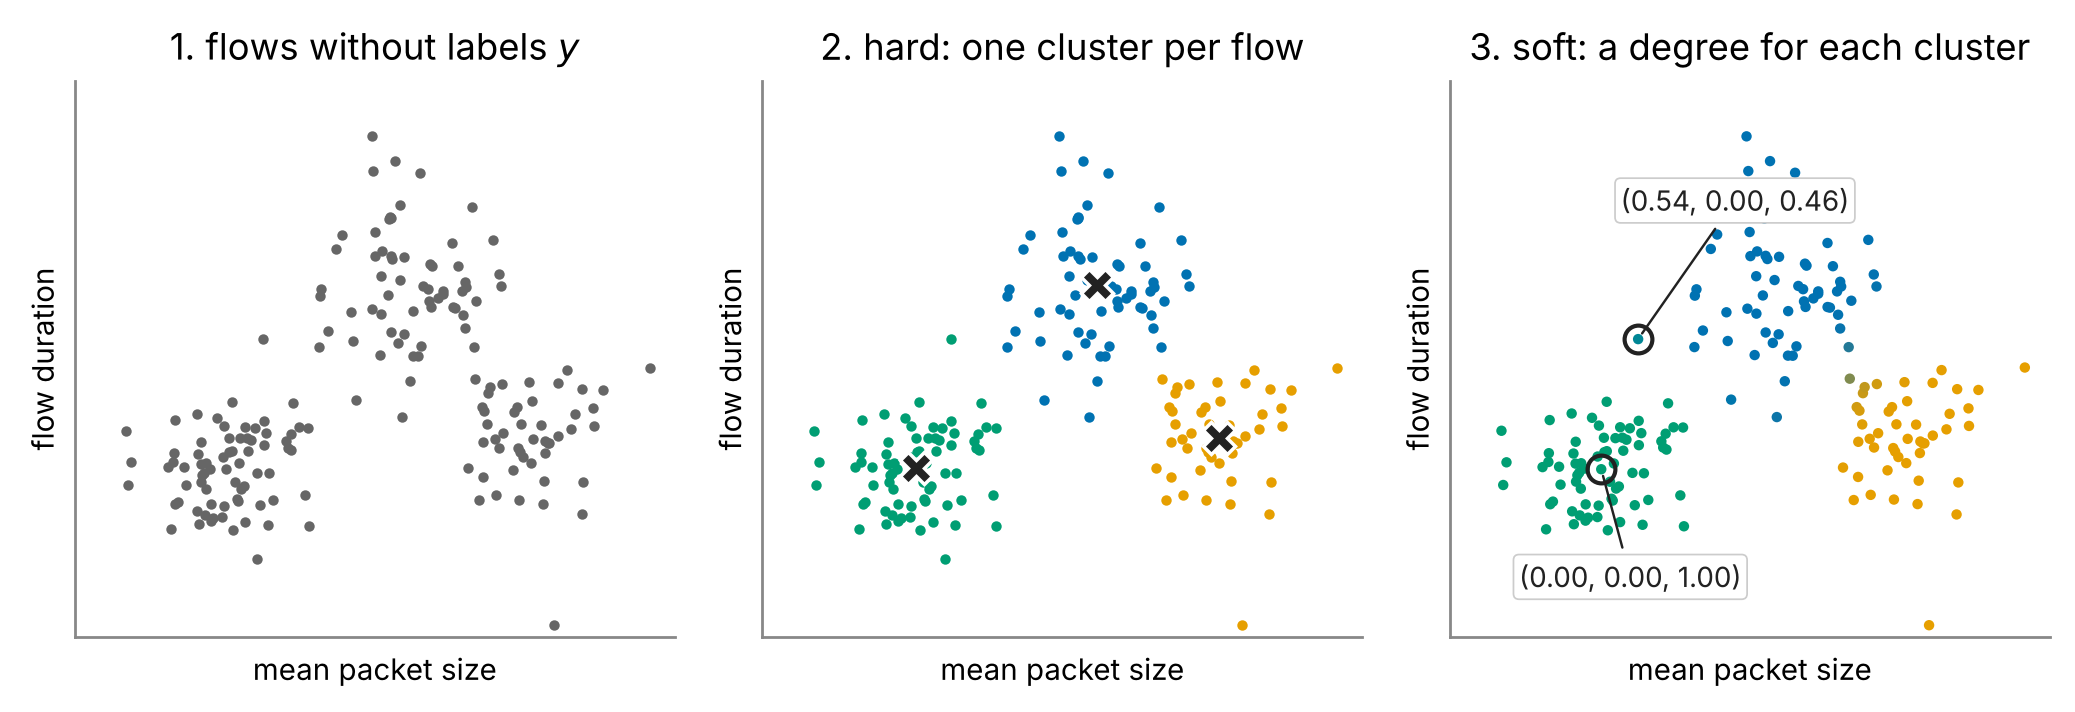
\includegraphics[width=1\textwidth]{images/chapter_10/clustering_intro.png}
    \caption{Clustering flows described by two features: the data have no labels; hard clustering gives each flow one cluster, soft clustering gives each flow a degree of belonging to every cluster.}
\end{figure}

\section{Hard Clustering}
Hard clustering techniques compute a predicted cluster index $\widehat{y}^{(i)} \in \{1, \dots, k\}$ (also written ${y'}^{(i)}$) for each data point, based solely on its feature vector $\mathbf{x}^{(i)}$. They do not require the true cluster index $y^{(i)}$ of any data point, and each data point is assigned to \textbf{only one} cluster. In the figure above, panel 2 is a hard clustering.

\subsection{k-Means}
The \textbf{k-Means} algorithm is a hard clustering algorithm characterized by one important parameter: the number of clusters $k$. Each cluster $c$ is represented by a point, its \textbf{mean} or \textbf{centroid} $\mathbf{m}^{(c)}$, which can be seen as the prototype feature vector of the cluster: the ``typical'' flow of that group.

A mean is a good representative when the points of the cluster are close to it, so it must be chosen carefully. The quality of a cluster $\mathcal{C}^{(c)}$ is measured by its \textbf{cluster spread}, the average squared Euclidean distance between its points and its mean:
\[
\text{spread}^{(c)} = \frac{1}{|\mathcal{C}^{(c)}|}\sum_{i \in \mathcal{C}^{(c)}} \big\|\mathbf{x}^{(i)} - \mathbf{m}^{(c)}\big\|^2 ,
\]
where $|\mathcal{C}^{(c)}|$ is the number of points in the cluster. The farther the points are from the mean, the larger the spread. The \textbf{clustering error} combines the spreads of all clusters:
\[
\mathcal{E}\big(\{\mathbf{m}^{(c)}\}, \{\widehat{y}^{(i)}\}\big) = \frac{1}{m}\sum_{c=1}^{k}\ \sum_{i \in \mathcal{C}^{(c)}} \big\|\mathbf{x}^{(i)} - \mathbf{m}^{(c)}\big\|^2 .
\]
It is the average, over all the $m$ data points, of the squared distance between each point and the mean of its cluster: the average of the cluster spreads, each weighted by the size of its cluster.\footnote{Correction: the previous version said that the clustering error is ``the sum of all spreads''. With the factor $1/m$ of the formula, it is the average of the spreads weighted by the cluster sizes, $\sum_c \frac{|\mathcal{C}^{(c)}|}{m}\,\text{spread}^{(c)}$, i.e. the average squared distance of a point from its mean.}

\paragraph{Minimizing the clustering error.} Two simple facts lead to the algorithm:
\begin{itemize}
    \item \textbf{for given cluster means}, the clustering error is minimized by assigning the $i$-th data point to the cluster with the \textbf{nearest cluster mean}, $\widehat{y}^{(i)} = \arg\min_{c}\|\mathbf{x}^{(i)} - \mathbf{m}^{(c)}\|$;
    \item \textbf{for given cluster assignments}, the clustering error is minimized by representing the $c$-th cluster with the \textbf{mean} of the feature vectors of its data points, $\mathbf{m}^{(c)} = \frac{1}{|\mathcal{C}^{(c)}|}\sum_{i \in \mathcal{C}^{(c)}} \mathbf{x}^{(i)}$.
\end{itemize}
Minimizing the clustering error is an ERM problem: we look for the cluster means $\mathbf{m}^{(c)}$ and the assignments $\widehat{y}^{(i)}$ that minimize it. Solving for both at the same time, exactly, is an NP-hard problem. The k-Means solution is an \textbf{alternating minimization}, in which the two easy problems above are solved one after the other, again and again. This is the core idea of k-Means.

\begin{center}
\fbox{\parbox{0.9\textwidth}{
\textbf{Algorithm: k-Means}\\
\textbf{Input:} feature vectors $\mathbf{x}^{(1)}, \dots, \mathbf{x}^{(m)}$, number of clusters $k$, initial cluster means (e.g. $k$ data points chosen at random)
\begin{enumerate}
    \item \textbf{Update cluster assignments}: assign each data point to the cluster with the nearest mean.
    \item \textbf{Update cluster means}: set each mean to the average of the points assigned to its cluster.
    \item Go to step 1, unless finished (the assignments, and hence the means, no longer change).
\end{enumerate}
\textbf{Output:} final cluster means $\mathbf{m}^{(c)}$ and cluster assignments $\widehat{y}^{(i)}$.}}
\end{center}

\begin{figure}[h]
    \centering
    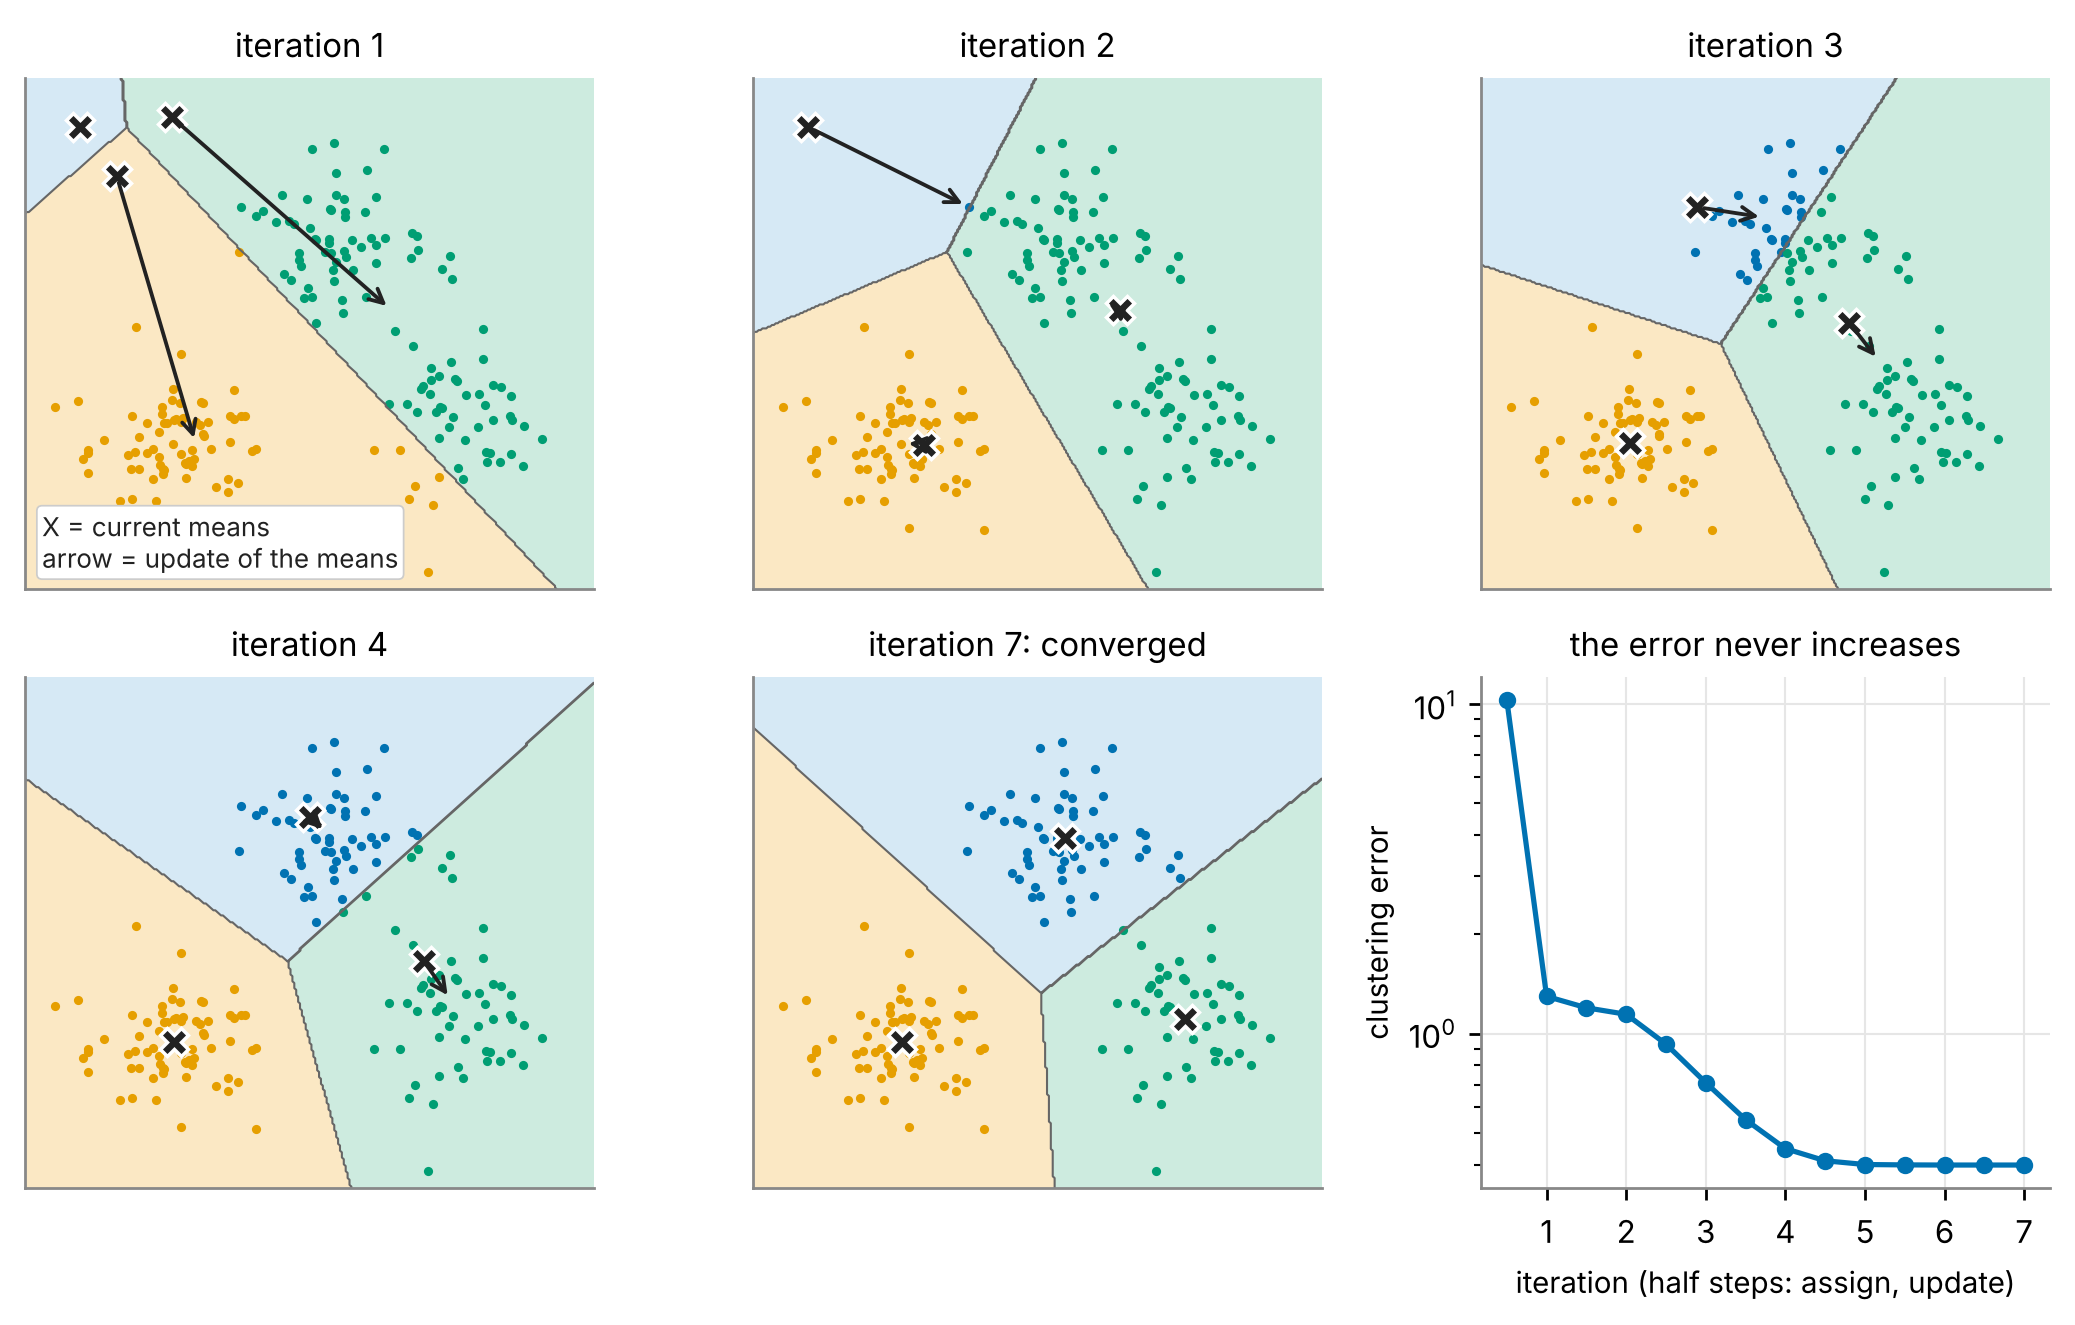
\includegraphics[width=1\textwidth]{images/chapter_10/kmeans_iterations.png}
    \caption{k-Means on 180 flows with $k = 3$ and a poor initialization (all means in the top-left corner). The coloured regions show the nearest-mean assignment, the arrows the update of the means. Bottom right: clustering error after each half step.}
\end{figure}

Additionally, k-Means has a very nice property: \textbf{k-Means never increases the clustering error}. Each of the two steps solves its own sub-problem optimally, so it cannot make the error larger:
\begin{itemize}
    \item each iteration produces new cluster means and assignments with a smaller or equal error, i.e. a smaller or equal empirical loss;\footnote{Correction: the previous version said that each iteration gives ``a smaller error''. The error can also stay the same, which is exactly what happens at convergence.}
    \item when the error stays constant, the algorithm has converged.
\end{itemize}
Hence, k-Means is an iterative optimization method. In the figure, starting from three means placed far from the data, the error drops from 10.3 to 1.3 with the first assignment and mean update, and after 7 iterations it settles at 0.40, with the three groups of flows correctly separated.

\subsection{Local Minima and Initialization}
When applying k-Means we must consider that the clustering error is \textbf{non-convex}: it has multiple local minima. k-Means, as every iterative method that only goes downhill, stops at the first minimum it finds. It may seem that we converged to the global minimum of the error, while in reality we reached a local minimum: k-Means stops when no single step can improve the clustering, but a completely different clustering may be much better.

\begin{figure}[h]
    \centering
    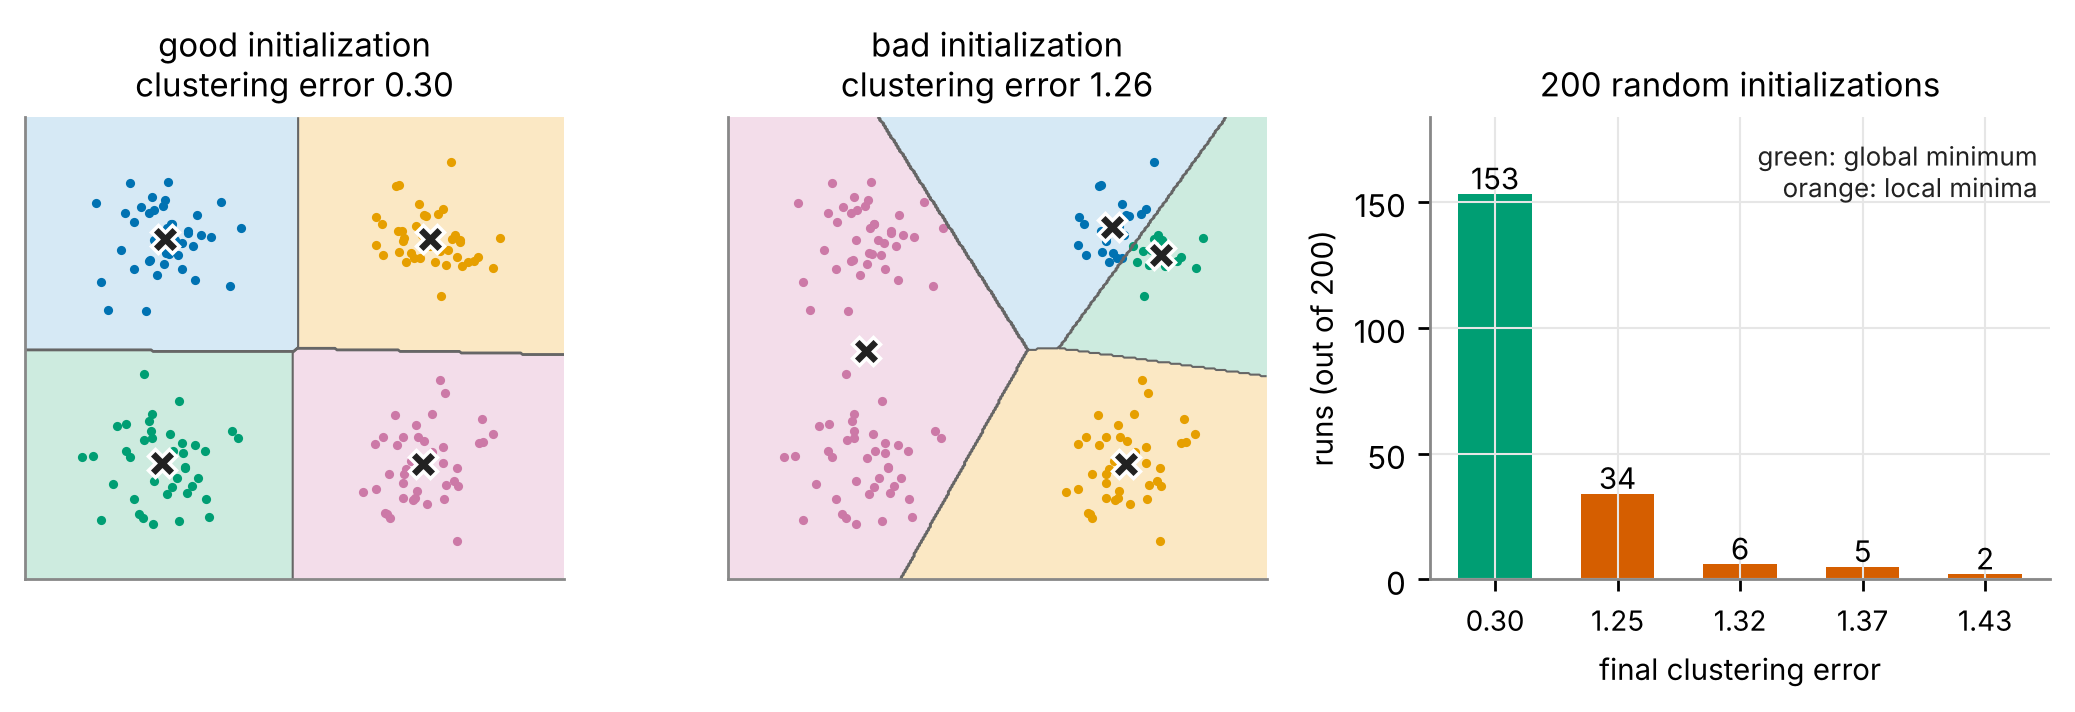
\includegraphics[width=1\textwidth]{images/chapter_10/kmeans_local_minima.png}
    \caption{k-Means with $k = 4$ on four well-separated groups. Left and centre: the result of a good and of a bad initialization. Right: final clustering error of 200 runs with random initial means.}
\end{figure}

With a bad initialization, two means start inside the same group and k-Means ends with one cluster split in two and two clusters merged into one: neither step can fix this, because moving one mean alone would increase the error. In the figure 153 runs out of 200 find the best clustering (error 0.30), while 47 runs end in a local minimum (error 1.25 to 1.43, four times larger). Since the results depend heavily on the initial means, it is recommended to \textbf{run k-Means several times} with different initial means and keep the clustering with the smallest error. With 200 runs the best one is found almost surely; scikit-learn's KMeans does this with the parameter n\_init, and also uses a smarter initialization (k-means++) that spreads the initial means apart.

\subsection{Choosing the Number of Clusters}
To choose the number of clusters $k$ we must consider that increasing $k$ can only decrease the (minimum) clustering error, which reaches 0 for $k = m$, when every point is its own cluster. So $k$ cannot be chosen by minimizing the error. Different strategies are used instead:
\begin{itemize}
    \item \textbf{defined by the application}: e.g. we want to separate 3 known traffic classes, or we have 5 operators who will each inspect one group of hosts;
    \item \textbf{desired compression rate}: each data point can be stored as the index of its cluster, which needs only $\log_2 k$ bits. A flow record with 20 features of 32 bits takes 640 bits; with $k = 256$ clusters it is replaced by an 8-bit index, a compression of 80 times, at the price of an error given by the clustering error;
    \item \textbf{elbow method}: plot the clustering error against $k$ and pick the value after which the gain from adding a cluster becomes negligible, similarly to the choice of the number of components in PCA;
    \item \textbf{validation error}: when clustering is used as pre-processing for a follow-up supervised problem (e.g. the cluster index becomes a new feature), try different values of $k$ and pick the one with the smallest validation error of the supervised problem.
\end{itemize}
The silhouette, described in the section on cluster validity, is another common criterion.

\begin{figure}[h]
    \centering
    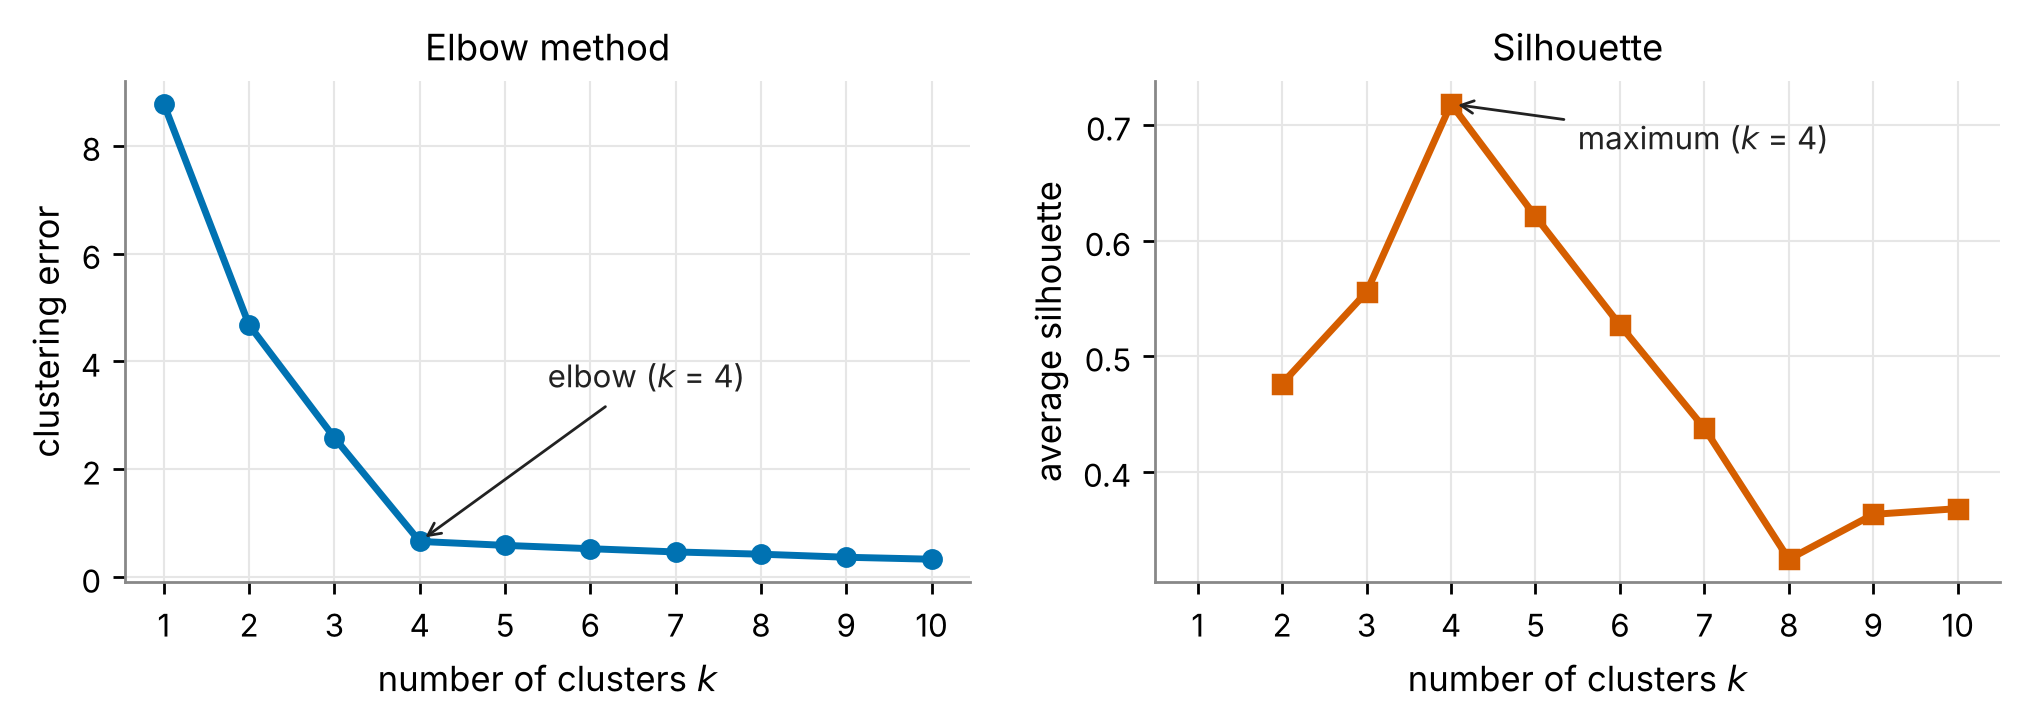
\includegraphics[width=1\textwidth]{images/chapter_10/elbow_silhouette.png}
    \caption{Choosing $k$ for 400 points in four groups: the clustering error has an elbow at $k = 4$, and the average silhouette is maximal at $k = 4$.}
\end{figure}

In the figure the error drops from 8.77 ($k = 1$) to 0.67 ($k = 4$), and then only to 0.59 for $k = 5$: the fifth cluster brings almost nothing, so $k = 4$ is the elbow. Real data rarely have such a clear elbow, which is why several criteria are usually combined.

\paragraph{To recap, k-Means:}
\begin{itemize}
    \item partitions the dataset into $k$ clusters, each represented by its mean;
    \item needs the number of clusters $k$ as a parameter;
    \item iteratively minimizes the clustering error, alternating assignments and means;
    \item might deliver a sub-optimal clustering (local minimum), therefore it must be repeated with different initial cluster means.
\end{itemize}

\section{Soft Clustering}
Soft clustering techniques do not assign each data point to a single cluster: they give the \textbf{degree} $\widehat{y}^{(i)}_c$ with which the $i$-th data point belongs to the $c$-th cluster. Hence, $\widehat{\mathbf{y}}^{(i)} = \big(\widehat{y}^{(i)}_1, \dots, \widehat{y}^{(i)}_k\big)$ is a vector containing the degree of belonging to each cluster, not a single index as in hard clustering. The degree can be interpreted as the probability that the $i$-th data point belongs to cluster $c$, so the degrees of each data point are between 0 and 1 and sum to 1. Hard clustering is the special case in which every $\widehat{y}^{(i)}_c$ is either 1 or 0.

Soft clustering is useful for points that lie between two groups. In the first figure of the chapter, the flow with degrees $(0.54, 0.00, 0.46)$ is almost equally close to two clusters, and the soft output says so honestly; a hard clustering would have to pick one of the two, hiding the doubt.

\subsection{Gaussian Mixture Model}
The \textbf{Gaussian Mixture Model} (GMM) represents each cluster $c$ as a multi-dimensional Gaussian distribution with its own mean $\boldsymbol{\mu}^{(c)}$ and covariance matrix $\boldsymbol{\Sigma}^{(c)}$, which contains the standard deviation of each feature and the correlations between features. Each cluster also has a weight, its \textbf{effective size} $m^{(c)} = \sum_{i} \widehat{y}^{(i)}_c$, the sum of the degrees of belonging of all points.\footnote{Correction: the previous version said that each Gaussian has its own ``mean, standard deviation and covariance matrix''. The standard deviations are already contained in the covariance matrix (on its diagonal); what is missing is the weight of each cluster, its effective size $m^{(c)}$.} The idea is that the points of a cluster are more likely near its centre and less likely on the edge of its ellipse. Unlike k-Means, whose clusters are implicitly round and of similar size, a GMM can describe clusters that are elongated, tilted, large or small.

\begin{figure}[h]
    \centering
    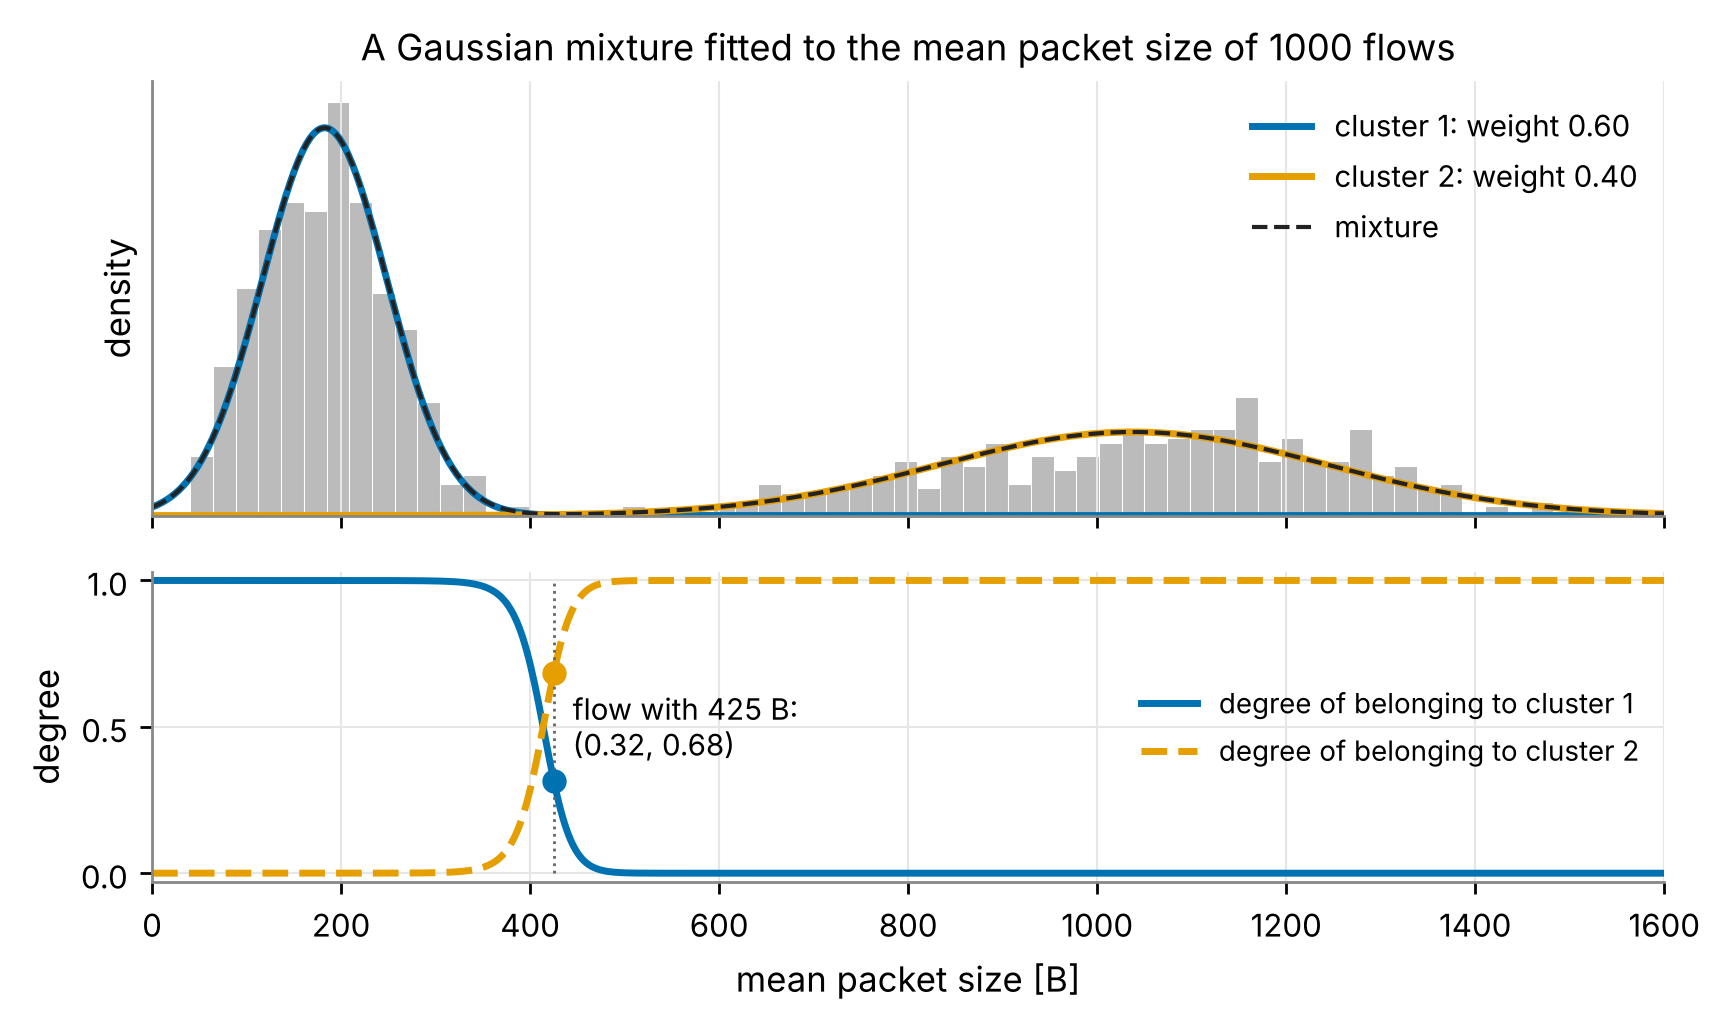
\includegraphics[width=0.85\textwidth]{images/chapter_10/gmm_1d.png}
    \caption{A GMM with two components fitted to the mean packet size of 1000 flows (small packets, e.g. interactive traffic, and large packets, e.g. bulk transfers). Bottom: degree of belonging to each cluster.}
\end{figure}

In the figure the two clusters have means $183$ and $1038$ bytes, standard deviations $66$ and $206$ bytes, and weights $0.60$ and $0.40$. A flow with mean packet size 425 B is closer to the first mean (242 B away) than to the second (613 B away), so k-Means would put it in cluster 1. The GMM gives it the degrees $(0.32, 0.68)$ instead, because 242 B is almost 4 standard deviations of the narrow cluster 1, while 613 B is only 3 standard deviations of the wide cluster 2. In a GMM, distances are measured relative to the spread of each cluster.

For this reason the cluster spread of a GMM weights each data point by its degree of belonging, and measures distances relative to the shape of the Gaussian:
\[
\text{spread}^{(c)} = \frac{1}{m^{(c)}}\sum_{i=1}^{m} \widehat{y}^{(i)}_c \big(\mathbf{x}^{(i)} - \boldsymbol{\mu}^{(c)}\big)^{T} \big(\boldsymbol{\Sigma}^{(c)}\big)^{-1} \big(\mathbf{x}^{(i)} - \boldsymbol{\mu}^{(c)}\big) .
\]
The product in the sum is the squared distance between the point and the mean, ``stretched'' according to the covariance matrix: a distance along the long axis of the ellipse counts less than the same distance along its short axis.

GMM also follows an iterative optimization, of the \textbf{soft-clustering error}
\[
\mathcal{E}\big(\{\boldsymbol{\mu}^{(c)}\}, \{\boldsymbol{\Sigma}^{(c)}\}, \{m^{(c)}\}\big) = -\sum_{i=1}^{m} \log \sum_{c=1}^{k} \frac{m^{(c)}}{m}\, p\big(\mathbf{x}^{(i)}; \boldsymbol{\mu}^{(c)}, \boldsymbol{\Sigma}^{(c)}\big) ,
\]
where $p(\mathbf{x}; \boldsymbol{\mu}, \boldsymbol{\Sigma})$ is the Gaussian density. The inner sum is the probability density of the point $\mathbf{x}^{(i)}$ under the whole mixture; the error is the negative logarithm of the probability of the whole dataset under the Gaussian mixture model, so minimizing it is equivalent to maximizing the (log) likelihood of the data. As in k-Means, the problem is solved by alternating two easy steps (this scheme is known as the \textbf{expectation-maximization}, EM, algorithm):

\begin{center}
\fbox{\parbox{0.9\textwidth}{
\textbf{Algorithm: GMM (expectation-maximization)}\\
\textbf{Input:} feature vectors $\mathbf{x}^{(1)}, \dots, \mathbf{x}^{(m)}$, number of clusters $k$, initial parameters $\boldsymbol{\mu}^{(c)}, \boldsymbol{\Sigma}^{(c)}, m^{(c)}$
\begin{enumerate}
    \item \textbf{Update the soft cluster assignments} $\widehat{y}^{(i)}_c$: for each point, the degree of cluster $c$ is proportional to $\frac{m^{(c)}}{m}\,p(\mathbf{x}^{(i)}; \boldsymbol{\mu}^{(c)}, \boldsymbol{\Sigma}^{(c)})$, normalized so that the degrees sum to 1.
    \item \textbf{Update the cluster parameters}: $m^{(c)} = \sum_i \widehat{y}^{(i)}_c$; $\boldsymbol{\mu}^{(c)}$ is the average of all points weighted by their degrees, $\frac{1}{m^{(c)}}\sum_i \widehat{y}^{(i)}_c\,\mathbf{x}^{(i)}$; $\boldsymbol{\Sigma}^{(c)}$ is their weighted covariance.
    \item Go to step 1, unless finished (the soft-clustering error no longer decreases).
\end{enumerate}
\textbf{Output:} degrees $\widehat{y}^{(i)}_c$ and cluster parameters $\boldsymbol{\mu}^{(c)}, \boldsymbol{\Sigma}^{(c)}, m^{(c)}$.}}
\end{center}
For given soft cluster assignments, the means and covariances are chosen to minimize the cluster spreads; for given parameters, the assignments are the probabilities of belonging. k-Means is a limit case of this algorithm, with degrees forced to be 0 or 1 and identical round clusters.

\begin{figure}[h]
    \centering
    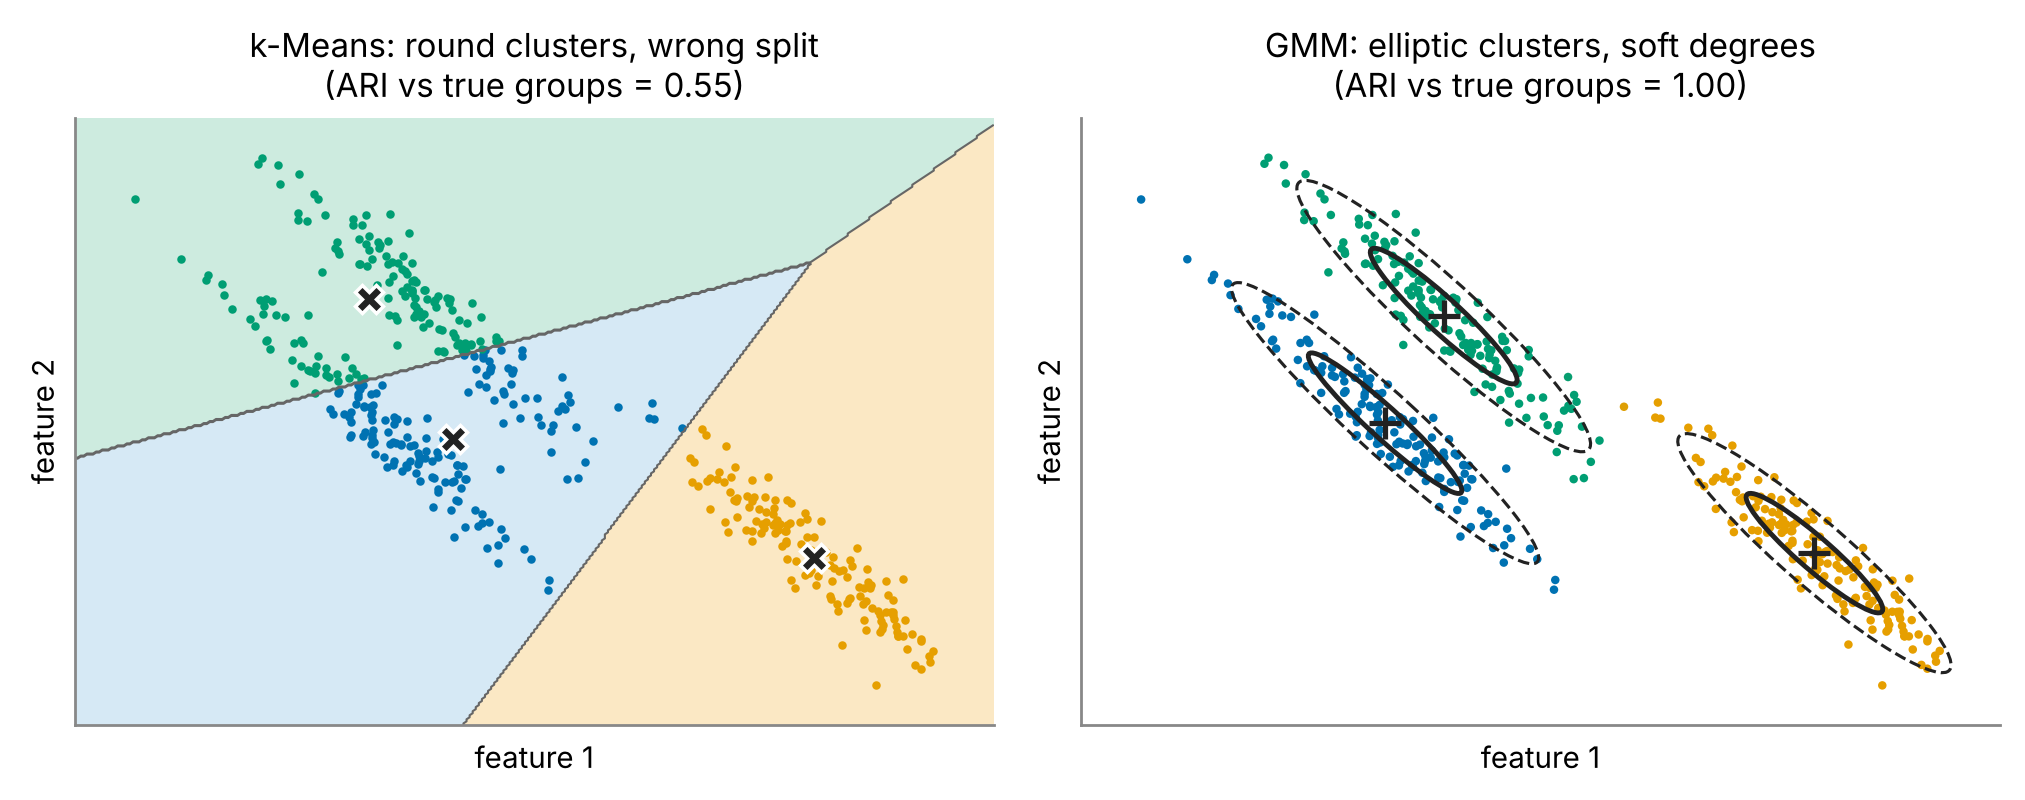
\includegraphics[width=1\textwidth]{images/chapter_10/kmeans_vs_gmm.png}
    \caption{Three elongated clusters. k-Means, which looks for round clusters, cuts them across; the GMM fits one ellipse to each (solid: 1 standard deviation, dashed: 2).}
\end{figure}

The same remarks on non-convexity of the clustering error, initialization and choice of $k$ made for k-Means apply to GMM. In the figure k-Means reaches an adjusted Rand index of only $0.55$ with respect to the true groups (the index is defined in the section on cluster validity), while the GMM recovers them perfectly ($1.00$).

\paragraph{To recap, GMM:}
\begin{itemize}
    \item represents each cluster by a Gaussian distribution (mean, covariance, weight) and gives each point a degree of belonging to each cluster;
    \item iteratively minimizes the soft-clustering error, alternating assignments and parameters;
    \item can be trapped in a local minimum by a bad initialization, so it is also repeated with different initial parameters.
\end{itemize}

\section{Other Clustering Approaches}
Both k-Means and GMM fail on clusters with complex shapes, e.g. curved or ring-shaped, because they describe each cluster by a centre and a round or elliptic spread.\footnote{Clarification: the previous version spoke of ``non-Euclidean cluster structures''. The distance used is still the Euclidean one; the problem is the shape of the clusters, which are not compact blobs around a centre (e.g. curved bands or rings).} In addition, they cannot recognize outliers and noise: every point, even an isolated one, is forced into some cluster, and it pulls that cluster's mean towards itself.

\begin{figure}[h]
    \centering
    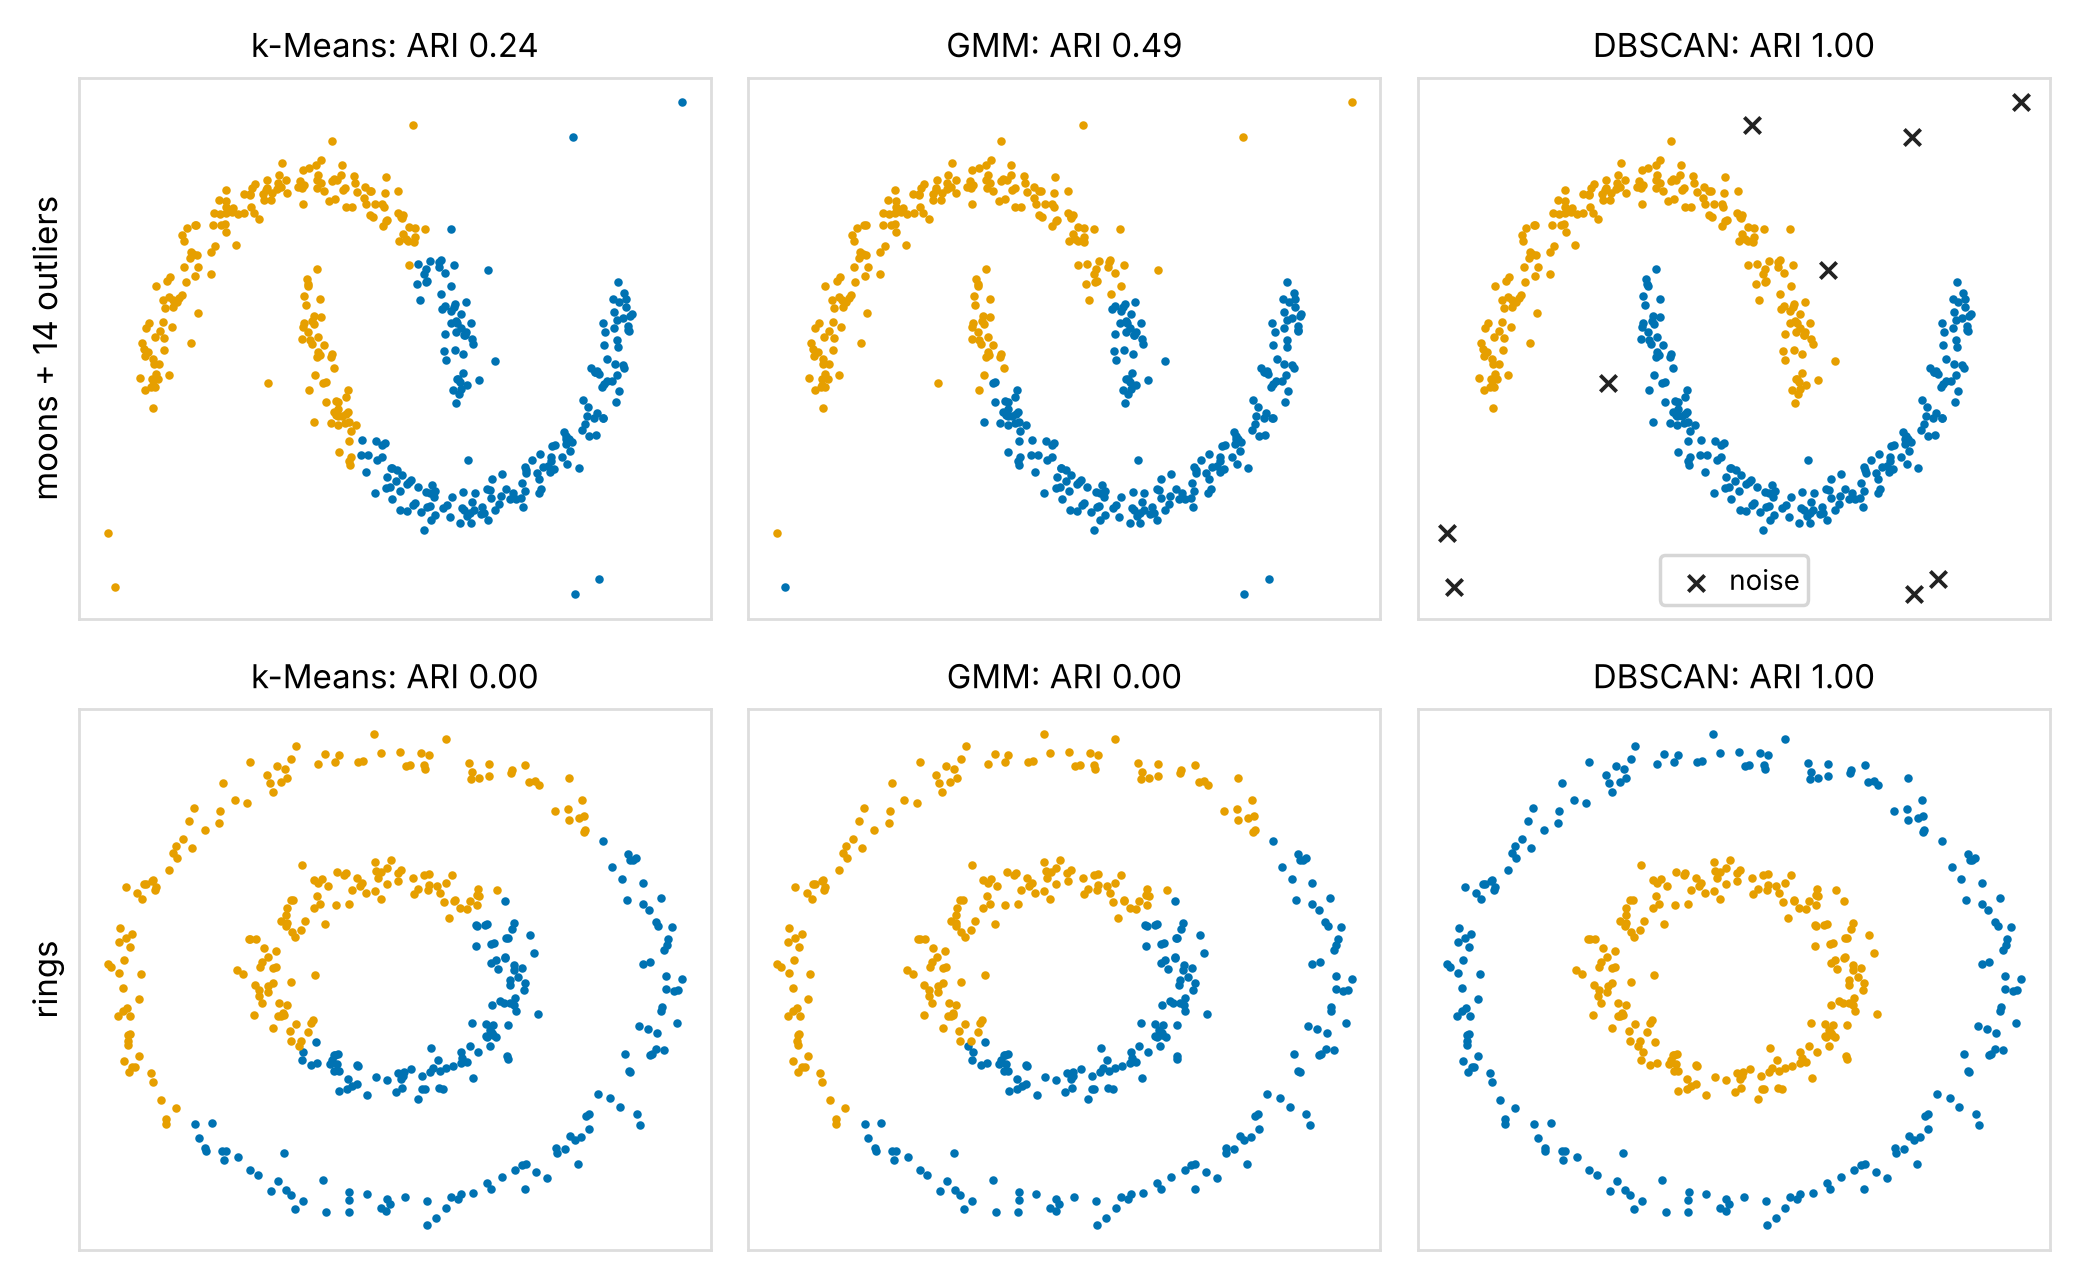
\includegraphics[width=1\textwidth]{images/chapter_10/failure_cases.png}
    \caption{Top: two curved clusters plus 14 random outliers. Bottom: two concentric rings. k-Means and GMM split the data with straight or elliptic boundaries; DBSCAN follows the shapes and marks most outliers as noise. ARI is computed on the non-outlier points.}
\end{figure}

\subsection{Connectivity Based Clustering}
Connectivity based clustering relies on the notion of \textbf{connectivity} between points: close-by data points are connected, as in a graph, and a cluster is a connected component of this graph, i.e. a set of points that can reach each other through a chain of close neighbours. Two points at the opposite ends of a curved cluster are far apart, but they belong to the same cluster because a chain of close points links them. This is why connectivity can follow any shape.

\textbf{DBSCAN} (density-based spatial clustering of applications with noise) is a hard clustering technique based on connectivity. It has two parameters: a radius $\varepsilon$ and a minimum number of points minPts. Points are classified as:
\begin{itemize}
    \item \textbf{core points}: points with at least minPts points (itself included) within distance $\varepsilon$, i.e. points inside a dense region;
    \item \textbf{border points}: points that are not core points but are within distance $\varepsilon$ of a core point, on the edge of a cluster;
    \item \textbf{noise points}: all the others, which are treated as outliers.
\end{itemize}
Clusters are made of core points connected to each other (two core points closer than $\varepsilon$ are in the same cluster), together with their border points.

\begin{figure}[h]
    \centering
    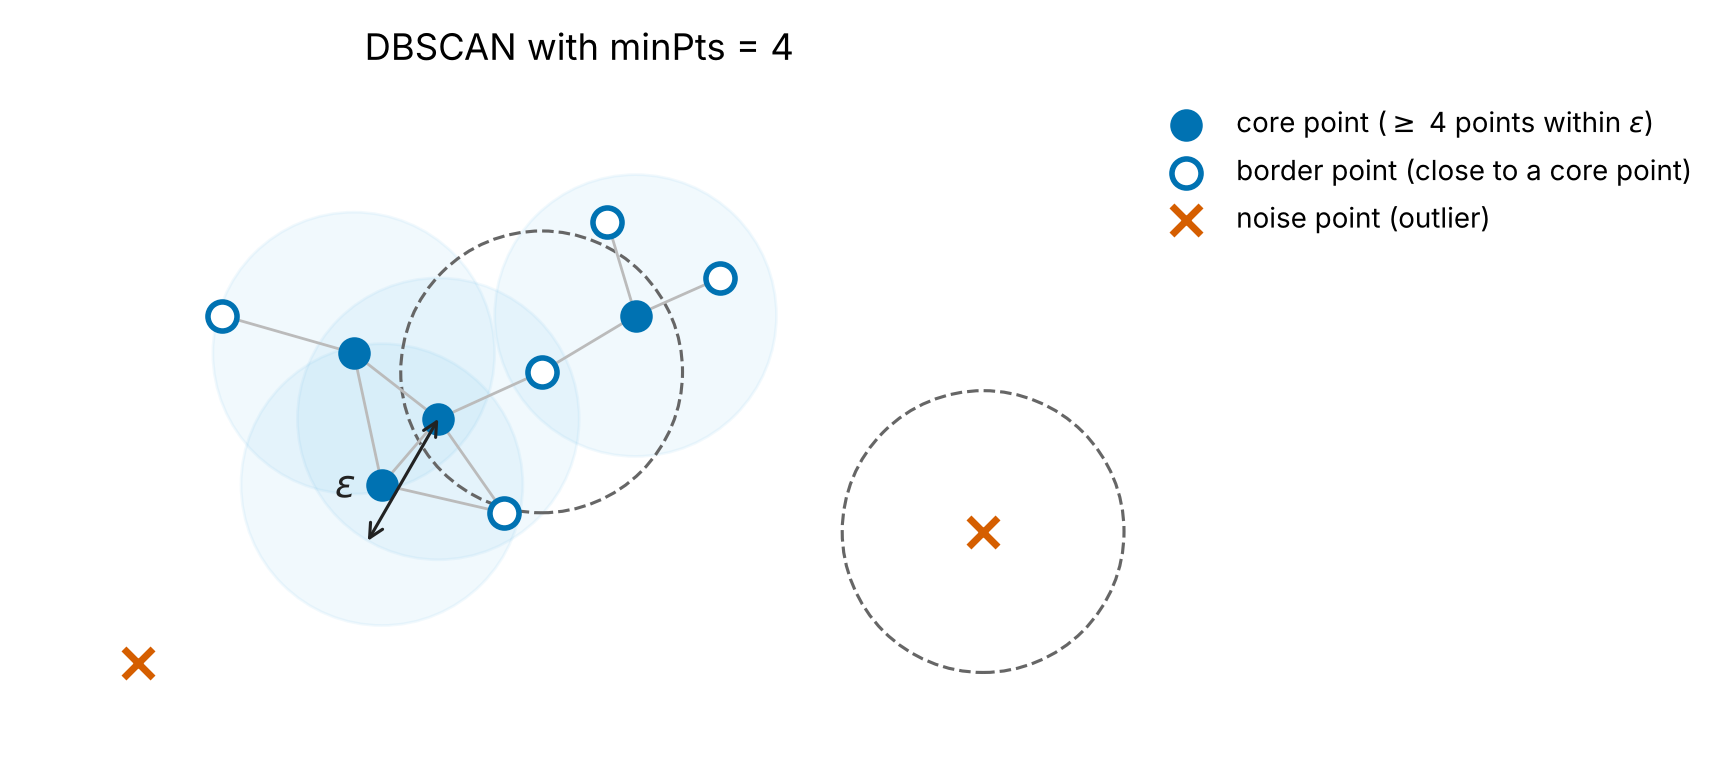
\includegraphics[width=0.8\textwidth]{images/chapter_10/dbscan_points.png}
    \caption{Core, border and noise points of DBSCAN with minPts $= 4$. The shaded discs have radius $\varepsilon$ around the core points; the dashed circles show that a border point and a noise point do not have enough neighbours.}
\end{figure}

DBSCAN \textbf{automatically determines the number of clusters} $k$, finds clusters of arbitrary shape and \textbf{labels outliers as noise}, which makes it well suited to anomaly detection: a host whose traffic does not resemble any group, e.g. a scanner contacting thousands of addresses, ends up as noise. In the figure with curved clusters it recovers both clusters perfectly and marks 9 of the 14 outliers as noise (the other 5 fall close to a cluster and are absorbed as border points). Its weak points are the choice of $\varepsilon$ and minPts, and clusters with very different densities, for which a single $\varepsilon$ does not fit all.

\subsection{Hierarchical Clustering}
Hierarchical clustering builds a set of \textbf{nested clusters}, organized as a hierarchical tree called a \textbf{dendrogram}. The usual (agglomerative) version starts with each point in its own cluster and repeatedly merges the two closest clusters, until a single cluster is left. Any desired number of clusters can then be obtained by \textbf{cutting the dendrogram} at the proper level: a horizontal cut crosses as many branches as the clusters it produces.

\begin{center}
\fbox{\parbox{0.9\textwidth}{
\textbf{Algorithm: agglomerative hierarchical clustering}\\
\textbf{Input:} feature vectors $\mathbf{x}^{(1)}, \dots, \mathbf{x}^{(m)}$, a proximity measure between clusters
\begin{enumerate}
    \item Start with $m$ clusters, one per data point.
    \item Find the two closest clusters and merge them; record the distance at which they merge.
    \item Repeat step 2 until a single cluster remains.
\end{enumerate}
\textbf{Output:} dendrogram; cut it at the desired height (or number of clusters).}}
\end{center}

\begin{figure}[h]
    \centering
    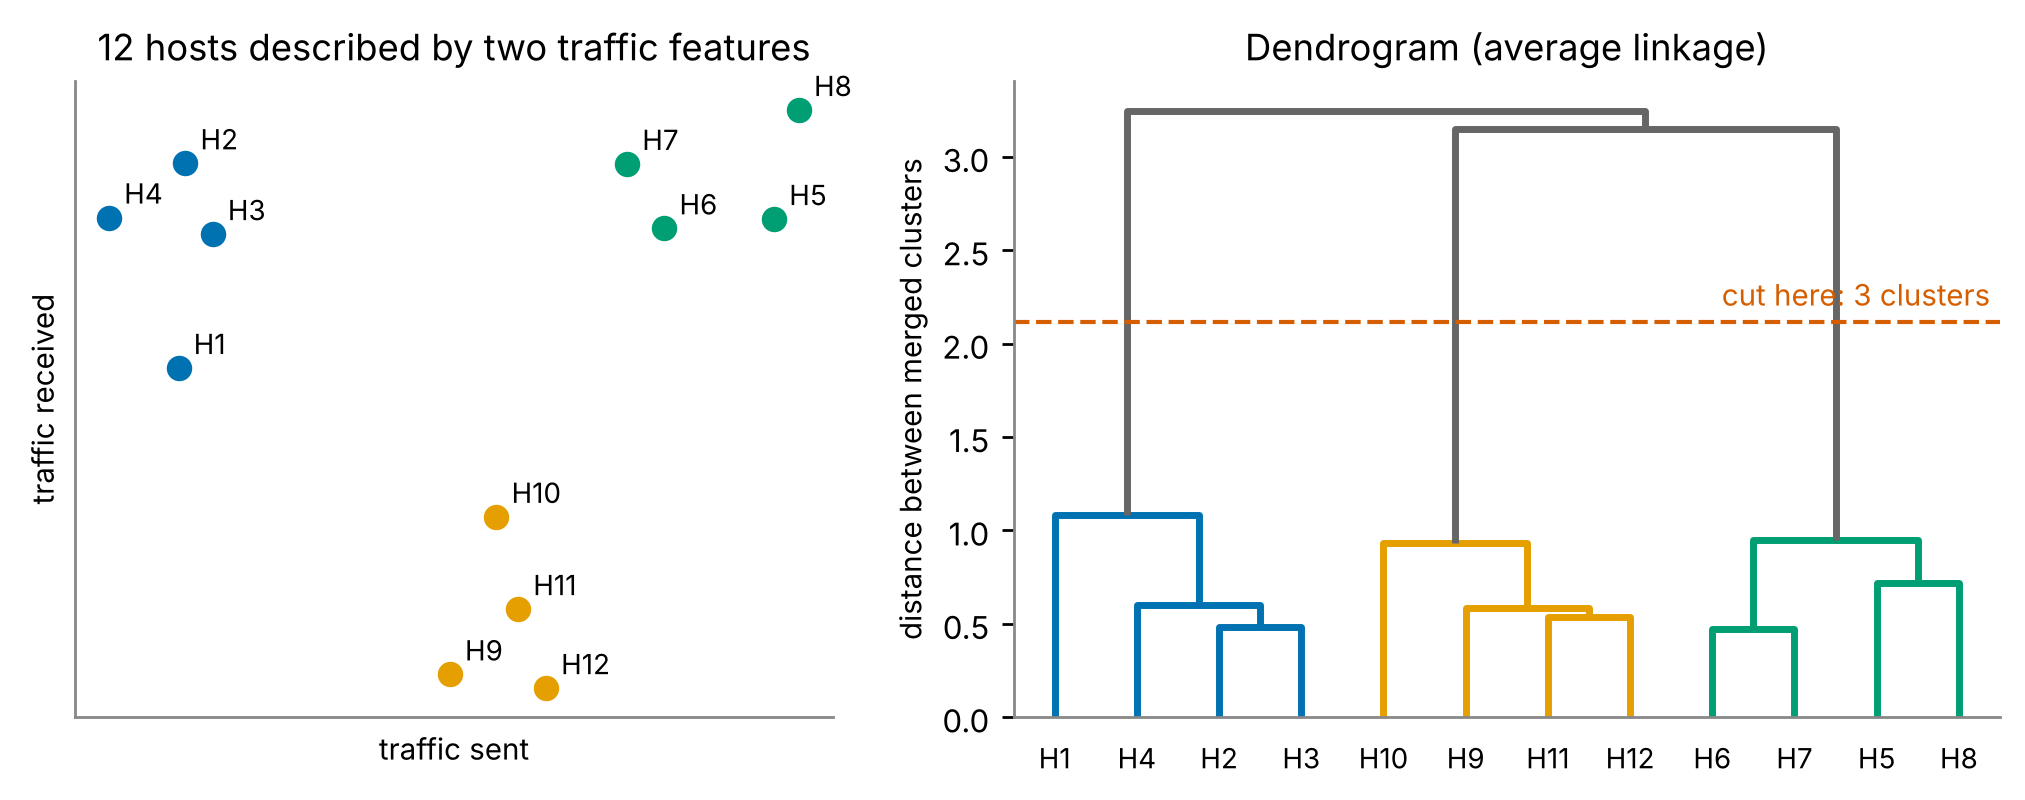
\includegraphics[width=1\textwidth]{images/chapter_10/dendrogram.png}
    \caption{Hierarchical clustering of 12 hosts. The height of each junction is the distance at which two clusters are merged; the dashed cut produces 3 clusters.}
\end{figure}

The key operation is the computation of the \textbf{proximity of 2 clusters}. Common choices are the distance between their two closest points (single linkage, which behaves like connectivity based clustering), between their two farthest points (complete linkage), or the average distance between their points (average linkage, used in the figure). In the dendrogram, long vertical branches before a merge mean well separated groups: here the three groups of hosts merge at heights below 1.1, while joining two groups requires a height above 3. Hierarchical clustering does not need $k$ in advance and gives a picture of the structure at all scales, but it needs the distances between all pairs of points, which is expensive for large datasets.

\begin{center}
    \begin{tabular}{l|c|c|l|l}
        & \textbf{Output} & \textbf{Needs $k$} & \textbf{Cluster shape} & \textbf{Outliers} \\ \hline
        k-Means      & hard & yes & round, similar size & forced into a cluster \\
        GMM          & soft & yes & elliptic            & forced into a cluster \\
        DBSCAN       & hard & no  & any (by density)    & labelled as noise \\
        Hierarchical & hard & no  & depends on linkage  & merged last \\
    \end{tabular}
\end{center}

\section{Measures of Cluster Validity}
Without labels, how do we know whether a clustering is good? Two kinds of measures exist:
\begin{itemize}
    \item \textbf{Internal index}: measures the goodness of a clustering structure without external information, using only the data and the clusters. Example: the \textbf{silhouette} index.
    \item \textbf{External or relative index}: measures the extent to which cluster labels match externally supplied class labels, or the labels of another clustering. Examples: \textbf{entropy}, \textbf{purity}, \textbf{Rand index} and \textbf{adjusted Rand index}.
\end{itemize}
External indices are useful to test a clustering method on data for which the true classes are known, e.g. a labelled traffic trace, before using it on unlabelled data.

\subsection{Silhouette}
The silhouette measures the consistency within clusters: how similar a data point is to its own cluster (\textbf{cohesion}) compared to the other clusters (\textbf{separation}). It is defined for each sample from two quantities:
\begin{itemize}
    \item $a$: the mean distance between the sample and all other points in the same cluster;
    \item $b$: the mean distance between the sample and all points in the next nearest cluster;
\end{itemize}
\[
s = \frac{b - a}{\max(a, b)} .
\]
If the point is much closer to its own cluster than to the next one ($a \ll b$), $s$ is close to $+1$; if it is equally close to both ($a \approx b$), $s$ is around 0; if it is closer to another cluster ($a > b$), $s$ is negative and the point is probably in the wrong cluster. For example, $a = 2$ and $b = 5$ give $s = 3/5 = 0.6$.

\begin{figure}[h]
    \centering
    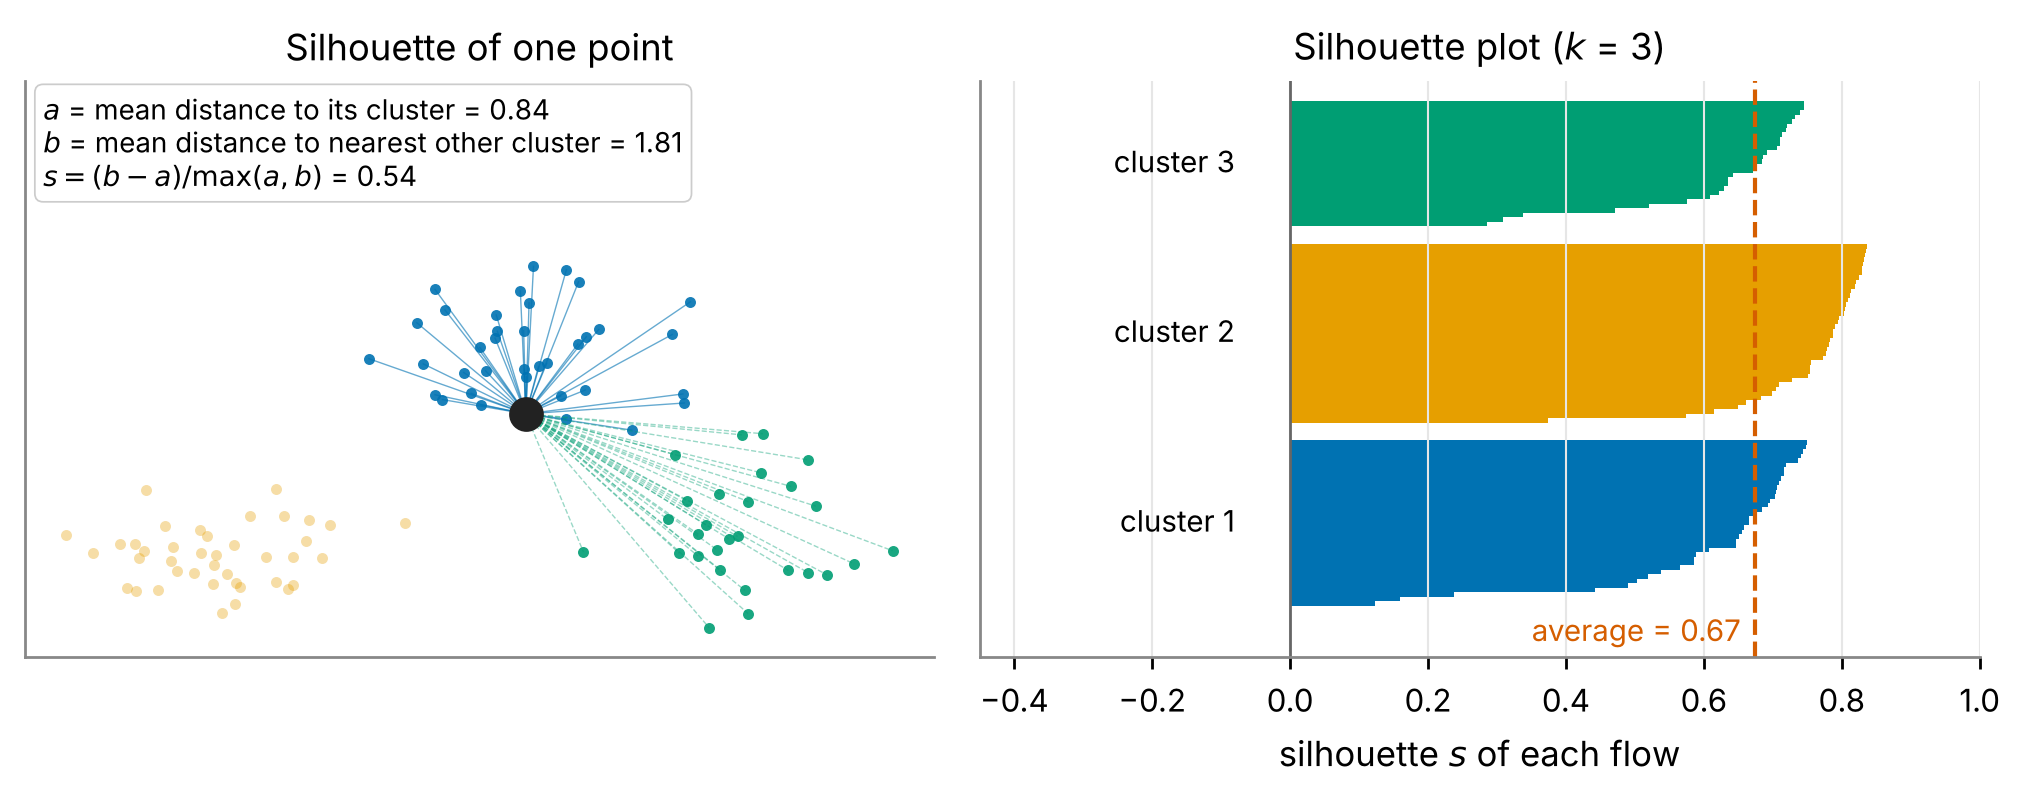
\includegraphics[width=1\textwidth]{images/chapter_10/silhouette.png}
    \caption{Left: $a$ and $b$ for one flow (solid lines: distances to its own cluster; dashed: to the nearest other cluster). Right: silhouette plot of all the flows, sorted within each cluster.}
\end{figure}

The main properties of the silhouette are:
\begin{itemize}
    \item the silhouette of a set of samples is the mean of the silhouettes of the samples;
    \item it ranges from $-1$ to $+1$: a high value indicates that the object is well matched to its own cluster and poorly matched to neighbouring clusters;
    \item scores around zero indicate overlapping clusters, negative scores indicate points assigned to the wrong cluster;
    \item if most objects have a high value, the clustering configuration is appropriate;
    \item it can be calculated with any distance metric;
    \item the average silhouette over the data of one cluster measures how tightly grouped the data in that cluster are, and the average over the whole dataset measures how appropriately the data have been clustered.
\end{itemize}
In the figure, the highlighted flow has $a = 0.84$ and $b = 1.81$, hence $s = (1.81 - 0.84)/1.81 = 0.54$. The average silhouette is $0.67$ and no flow has a negative value. The average silhouette can also be used to choose $k$, as in the elbow figure: it is highest when the clusters are both compact and well separated.

\subsection{Entropy and Purity}
When true classes are available, each cluster can be compared with them:
\begin{itemize}
    \item \textbf{purity}: each cluster is labelled with its most frequent class, and purity is the fraction of points that belong to that majority class. A cluster with 8 web flows and 2 video flows has purity $0.8$; purity 1 means that every cluster contains a single class;
    \item \textbf{entropy}: measures how mixed the classes are inside each cluster; it is 0 when each cluster contains a single class and grows as the classes get mixed. The entropy of the clustering is the average of the cluster entropies, weighted by the cluster sizes.
\end{itemize}
Both are easily fooled by many clusters: with one cluster per point, purity is 1 and entropy is 0.

\subsection{Rand Index}
The \textbf{Rand index} (RI) measures the similarity of two assignments, e.g. a clustering and the true classes, or two clusterings. Instead of comparing the labels, which are arbitrary names (cluster 1 of one clustering may correspond to cluster 3 of the other), it looks at \textbf{pairs} of points. Given a dataset $\mathcal{D}$ with $m$ elements and two partitions $S$ and $R$:
\begin{itemize}
    \item $a$ is the number of pairs of elements of $\mathcal{D}$ that are in the same subset in $S$ and in the same subset in $R$;
    \item $b$ is the number of pairs of elements of $\mathcal{D}$ that are in different subsets in $S$ and in different subsets in $R$.
\end{itemize}
The number of all possible pairs of elements of $\mathcal{D}$ is the binomial coefficient $\binom{m}{2} = m(m-1)/2$, and
\[
RI(S, R) = \frac{a + b}{\binom{m}{2}} .
\]
The numerator counts the pairs on which the two partitions agree (``together'' in both, or ``apart'' in both). The Rand index can be interpreted as an accuracy: it is the fraction of pairs on which the two partitions take the same decision.\footnote{Clarification: the previous version said only that ``Rand Index can be interpreted as accuracy''. It is the accuracy of the pairwise decisions ``same cluster / different cluster'', not of the labels themselves, which may be named differently in the two partitions.} It is 1 when the partitions are identical.

\subsection{Adjusted Rand Index}
The Rand index does not ensure a value close to 0 for a random labelling. With many clusters, most pairs are ``apart'' in both partitions just by chance, and $b$ alone makes RI large. The \textbf{adjusted Rand index} (ARI) corrects for chance and provides a baseline:
\[
ARI = \frac{RI - \mathrm{E}[RI]}{\max(RI) - \mathrm{E}[RI]} ,
\]
where $\mathrm{E}[RI]$ is the value expected for random partitions with the same cluster sizes. ARI is 1 for identical partitions, about 0 for random ones, and can even be negative.

\begin{figure}[h]
    \centering
    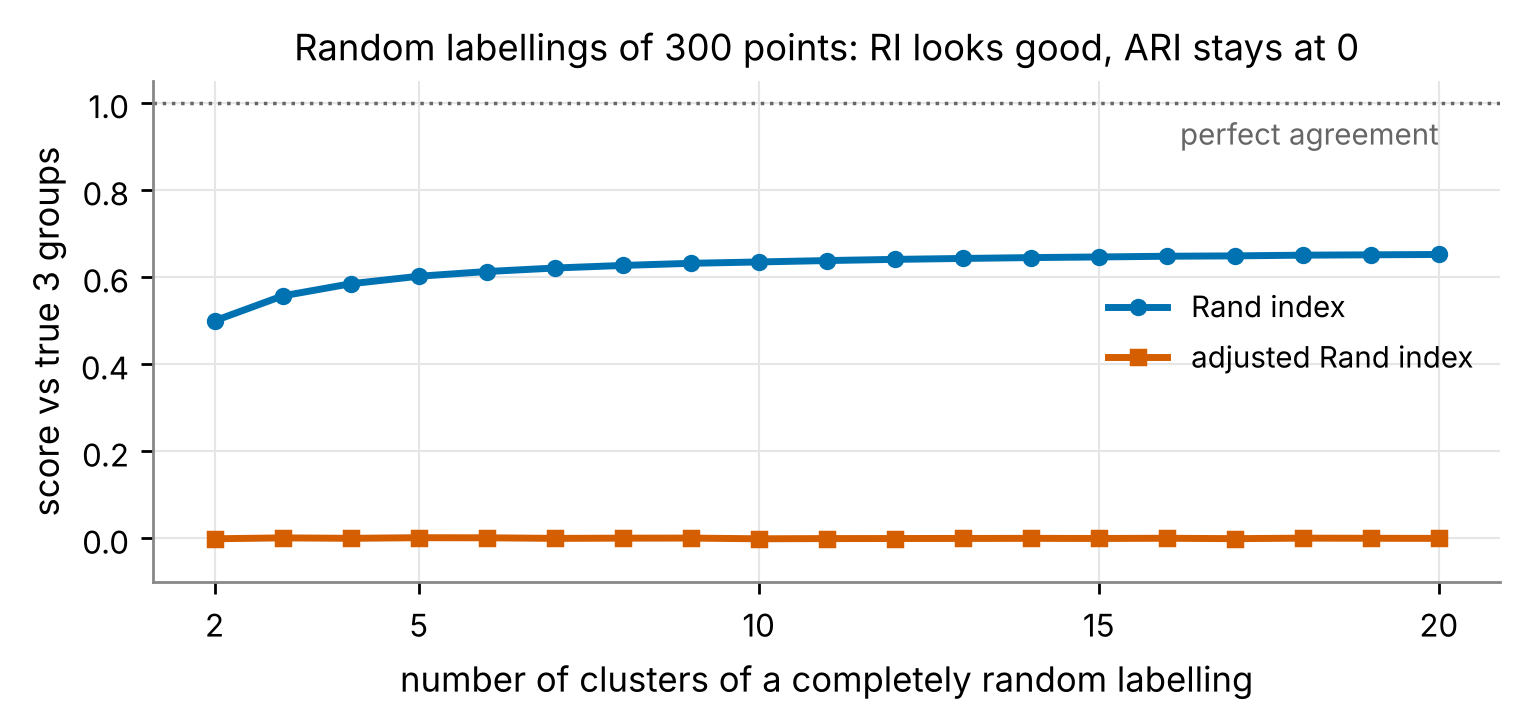
\includegraphics[width=0.75\textwidth]{images/chapter_10/ri_vs_ari.png}
    \caption{Completely random labellings of 300 points compared with their 3 true groups: the Rand index is between 0.5 and 0.65, the adjusted Rand index stays at 0.}
\end{figure}

\section{Self-Assessment Quiz}
The chapter ends with three exercises on the following dataset with 9 samples and 1 feature: $10, 7, 7, 5, -1, 10, 2, -3, 0$.

\paragraph{1. Possible outputs of a hard and of a soft clustering method with 3 clusters.} A hard clustering gives one index per sample. k-Means with $k = 3$ finds the means $10$, $6.33$ and $-0.5$, with assignments $(1, 2, 2, 2, 3, 1, 3, 3, 3)$: the samples $\{10, 10\}$, $\{7, 7, 5\}$ and $\{-1, 2, -3, 0\}$. A soft clustering gives a vector of 3 degrees per sample, summing to 1. A GMM with 3 components finds clusters with the same means, and is almost certain for every sample: for example sample $10$ gets $(1.00, 0.00, 0.00)$. The least certain sample is $5$, the one between two groups, with degrees $(0.00, 0.98, 0.02)$.

\paragraph{2. Up to 5 iterations of k-Means with $k = 2$.} Taking the first two samples as initial means, $10$ and $7$:
\begin{center}
    \begin{tabular}{c|c|l|l|c|c}
        \textbf{Iter.} & \textbf{Means used} & \textbf{Cluster 1} & \textbf{Cluster 2} & \textbf{New means} & \textbf{Error} \\ \hline
        1 & $10$, $7$     & $10, 10$             & $7, 7, 5, -1, 2, -3, 0$ & $10$, $2.43$  & $10.63$ \\
        2 & $10$, $2.43$  & $10, 7, 7, 10$       & $5, -1, 2, -3, 0$       & $8.5$, $0.6$  & $5.13$ \\
        3 & $8.5$, $0.6$  & $10, 7, 7, 5, 10$    & $-1, 2, -3, 0$          & $7.8$, $-0.5$ & $3.53$ \\
        4 & $7.8$, $-0.5$ & $10, 7, 7, 5, 10$    & $-1, 2, -3, 0$          & $7.8$, $-0.5$ & $3.53$ \\
    \end{tabular}
\end{center}
Each sample goes to the nearest mean, i.e. to cluster 1 when it is above the midpoint between the two means ($8.5$, then $6.21$, then $4.55$). In iteration 1, for instance, cluster 2 gets $7, 7, 5, -1, 2, -3, 0$, whose mean is $17/7 = 2.43$. In iteration 4 the assignments do not change, so k-Means has converged after 4 of the 5 allowed iterations. The error, computed with the formula of the clustering error, decreases at every iteration, as expected: in iteration 3, for example, the squared distances are $2.2^2 + 0.8^2 + 0.8^2 + 2.8^2 + 2.2^2 = 18.8$ in cluster 1 and $0.5^2 + 2.5^2 + 2.5^2 + 0.5^2 = 13$ in cluster 2, so $\mathcal{E} = (18.8 + 13)/9 = 3.53$.

\begin{figure}[h]
    \centering
    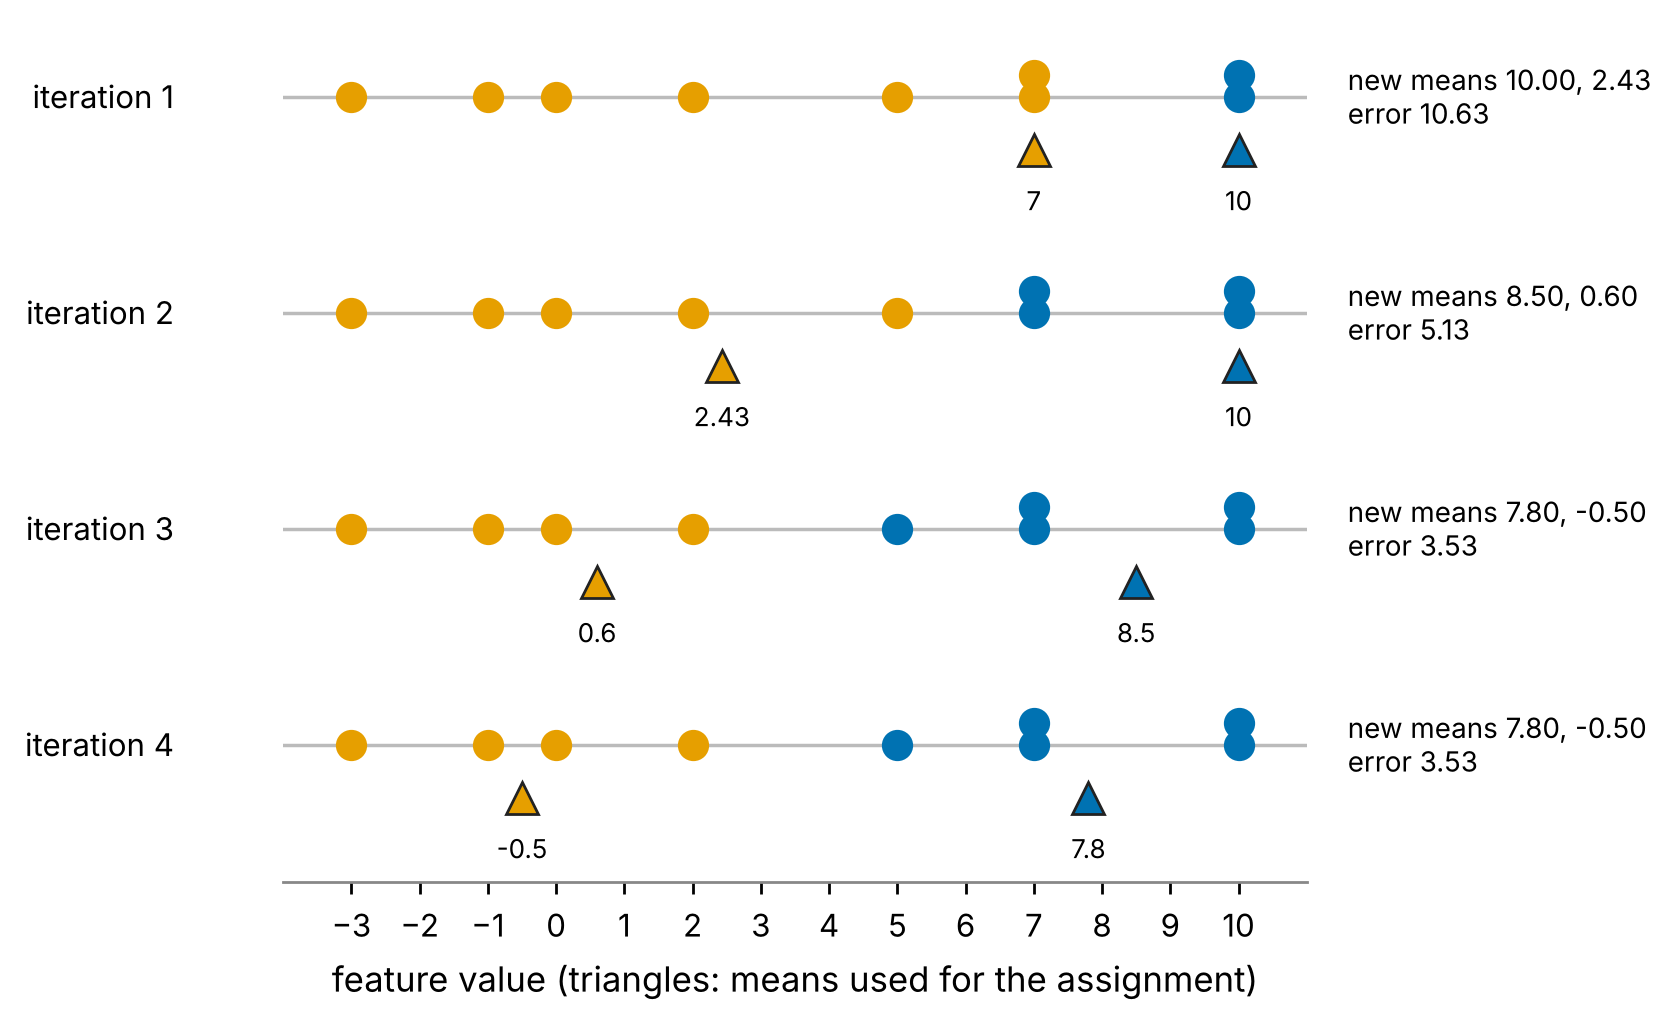
\includegraphics[width=0.8\textwidth]{images/chapter_10/kmeans_quiz.png}
    \caption{The iterations of the quiz: samples coloured by their cluster, triangles at the means used for the assignment.}
\end{figure}

\paragraph{3. Rand index with respect to the assignment $(0,0,0,0,0,0,0,1,1)$.} The k-Means result is $S = (0,0,0,0,1,0,1,1,1)$, with 0 for the cluster with mean $7.8$, and the given assignment is $R = (0,0,0,0,0,0,0,1,1)$. Out of the $\binom{9}{2} = 36$ pairs:
\begin{itemize}
    \item $a = 12$ pairs are together in both: the $\binom{5}{2} = 10$ pairs among samples 1, 2, 3, 4, 6, the pair (5, 7) and the pair (8, 9);
    \item $b = 10$ pairs are apart in both: each of the samples 1, 2, 3, 4, 6 with each of the samples 8, 9;
    \item the remaining $14$ pairs disagree.
\end{itemize}
Hence $RI = (12 + 10)/36 = 0.61$. The adjusted Rand index is only $0.24$: the two partitions agree a little more than chance would predict, but not much.

\begin{figure}[h]
    \centering
    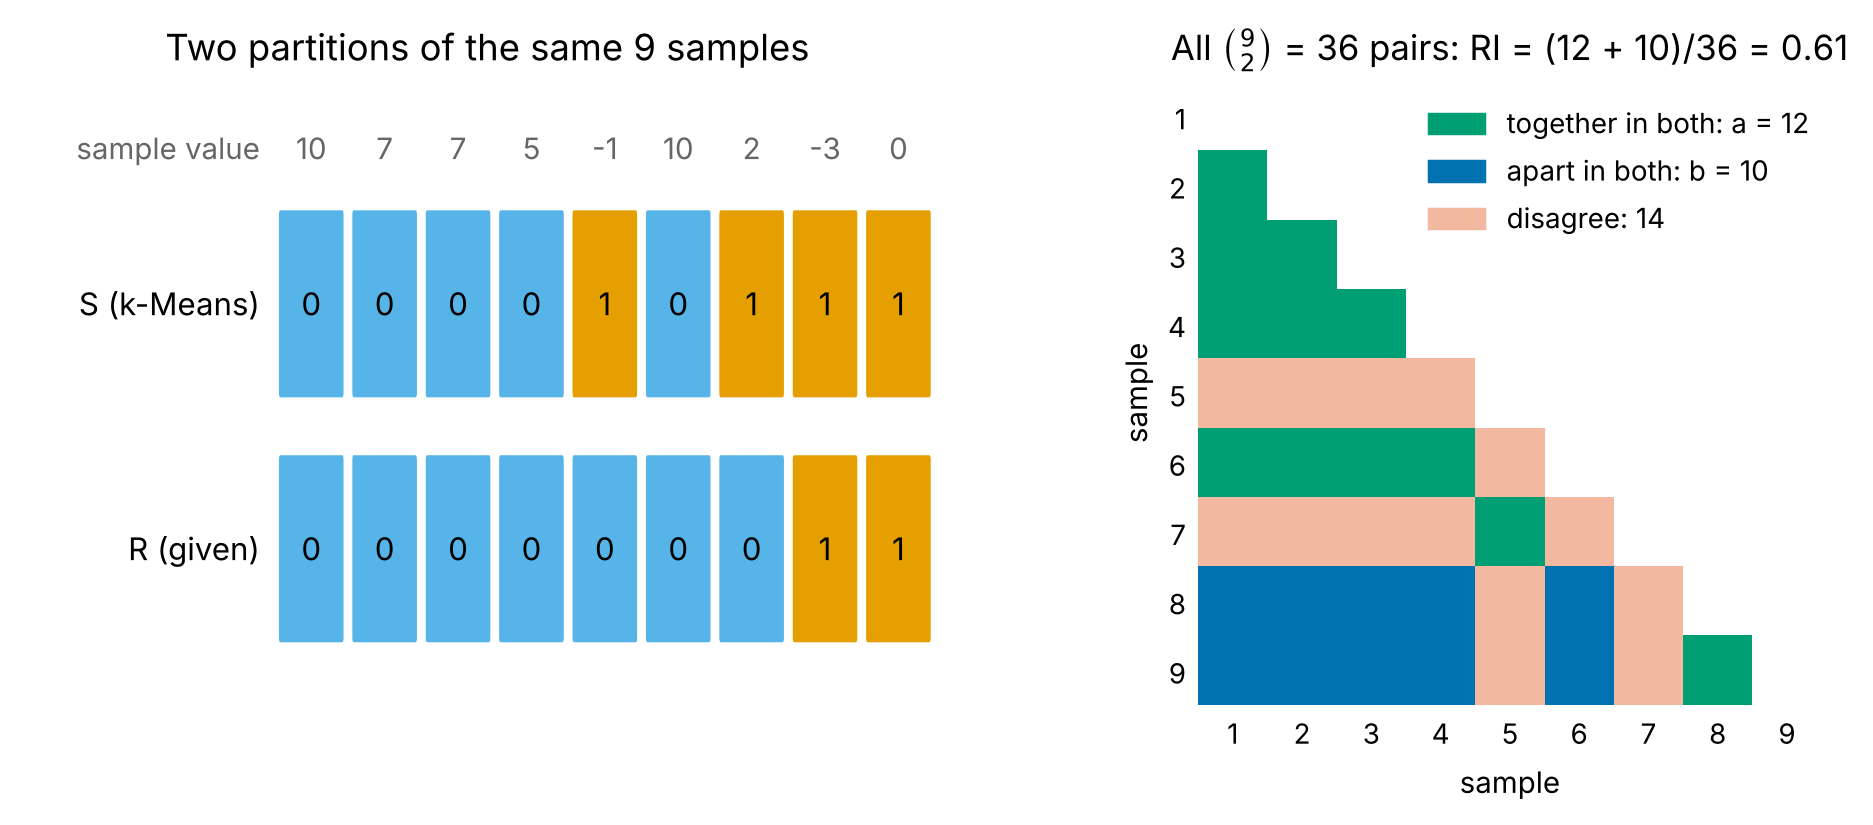
\includegraphics[width=0.95\textwidth]{images/chapter_10/rand_index.png}
    \caption{Pair counting for the Rand index of the quiz: each cell of the triangle is a pair of samples.}
\end{figure}

\section{Summary}
\begin{itemize}
    \item Clustering groups unlabelled data points into homogeneous groups. \textbf{Hard} clustering gives one cluster per point, \textbf{soft} clustering a degree of belonging to each cluster.
    \item \textbf{k-Means} represents each cluster by its mean and minimizes the clustering error by alternating two steps: assign each point to the nearest mean, move each mean to the average of its points. The error never increases, but the algorithm can stop in a local minimum, so it is run with several initializations.
    \item $k$ is chosen by the application, the compression rate, the elbow method, the silhouette, or the validation error of a follow-up supervised problem.
    \item \textbf{GMM} represents each cluster by a Gaussian (mean, covariance, weight), fits elliptic clusters and gives soft degrees; it minimizes the negative log-likelihood with the EM algorithm.
    \item \textbf{DBSCAN} builds clusters of any shape from connected dense regions, finds $k$ by itself and labels outliers as noise. \textbf{Hierarchical clustering} builds a dendrogram that can be cut at any number of clusters.
    \item Validity: the \textbf{silhouette} $s = (b-a)/\max(a,b)$ needs no labels; \textbf{purity}, \textbf{entropy}, \textbf{Rand index} and \textbf{adjusted Rand index} compare the clustering with known classes. ARI corrects the Rand index for chance.
\end{itemize}



\section{A prova di coglione}
Fin qui avevamo sempre le etichette: questo flusso è web, quest'altro è un attacco. Nel clustering le etichette non ci sono, e il compito è trovare da soli i gruppi di dati simili tra loro. Nel networking serve a scoprire quali tipi di traffico ci sono in una rete senza etichettare niente a mano, a raggruppare host con comportamenti simili e a scovare chi non somiglia a nessuno, cioè le anomalie.

\subsection{k-Means: gruppi rotondi attorno a un centro}
\paragraph*{L'idea.} Ogni gruppo ha un centro, la media dei suoi punti, e ogni punto va con il centro più vicino. È come decidere dove mettere $k$ pizzerie in una città: ogni cliente va in quella più vicina, e ogni pizzeria si sposta al centro dei suoi clienti.

L'algoritmo alterna due passi semplici: assegna ogni punto al centro più vicino, poi sposta ogni centro nella media dei suoi punti, e ripete finché non cambia più niente. L'errore da minimizzare è la distanza media (al quadrato) tra ogni punto e il suo centro, e ogni passo non può che abbassarlo o lasciarlo uguale.

Il problema è che k-Means si ferma al primo minimo che trova. Se due centri partono nello stesso gruppo, finisce con un gruppo spezzato in due e due gruppi fusi in uno, e da lì non si sposta più. Nell'esempio del capitolo succede in 47 partenze casuali su 200. La soluzione è semplice: lo si fa girare tante volte e si tiene il risultato con l'errore più basso.

Il valore di $k$ non si sceglie minimizzando l'errore, perché più gruppi fai e più l'errore scende, fino a zero con un gruppo per punto. Si usa il gomito, cioè il punto dopo il quale aggiungere un gruppo non migliora quasi niente, oppure la silhouette, oppure le esigenze dell'applicazione.

\begin{figure}[h]
    \centering
    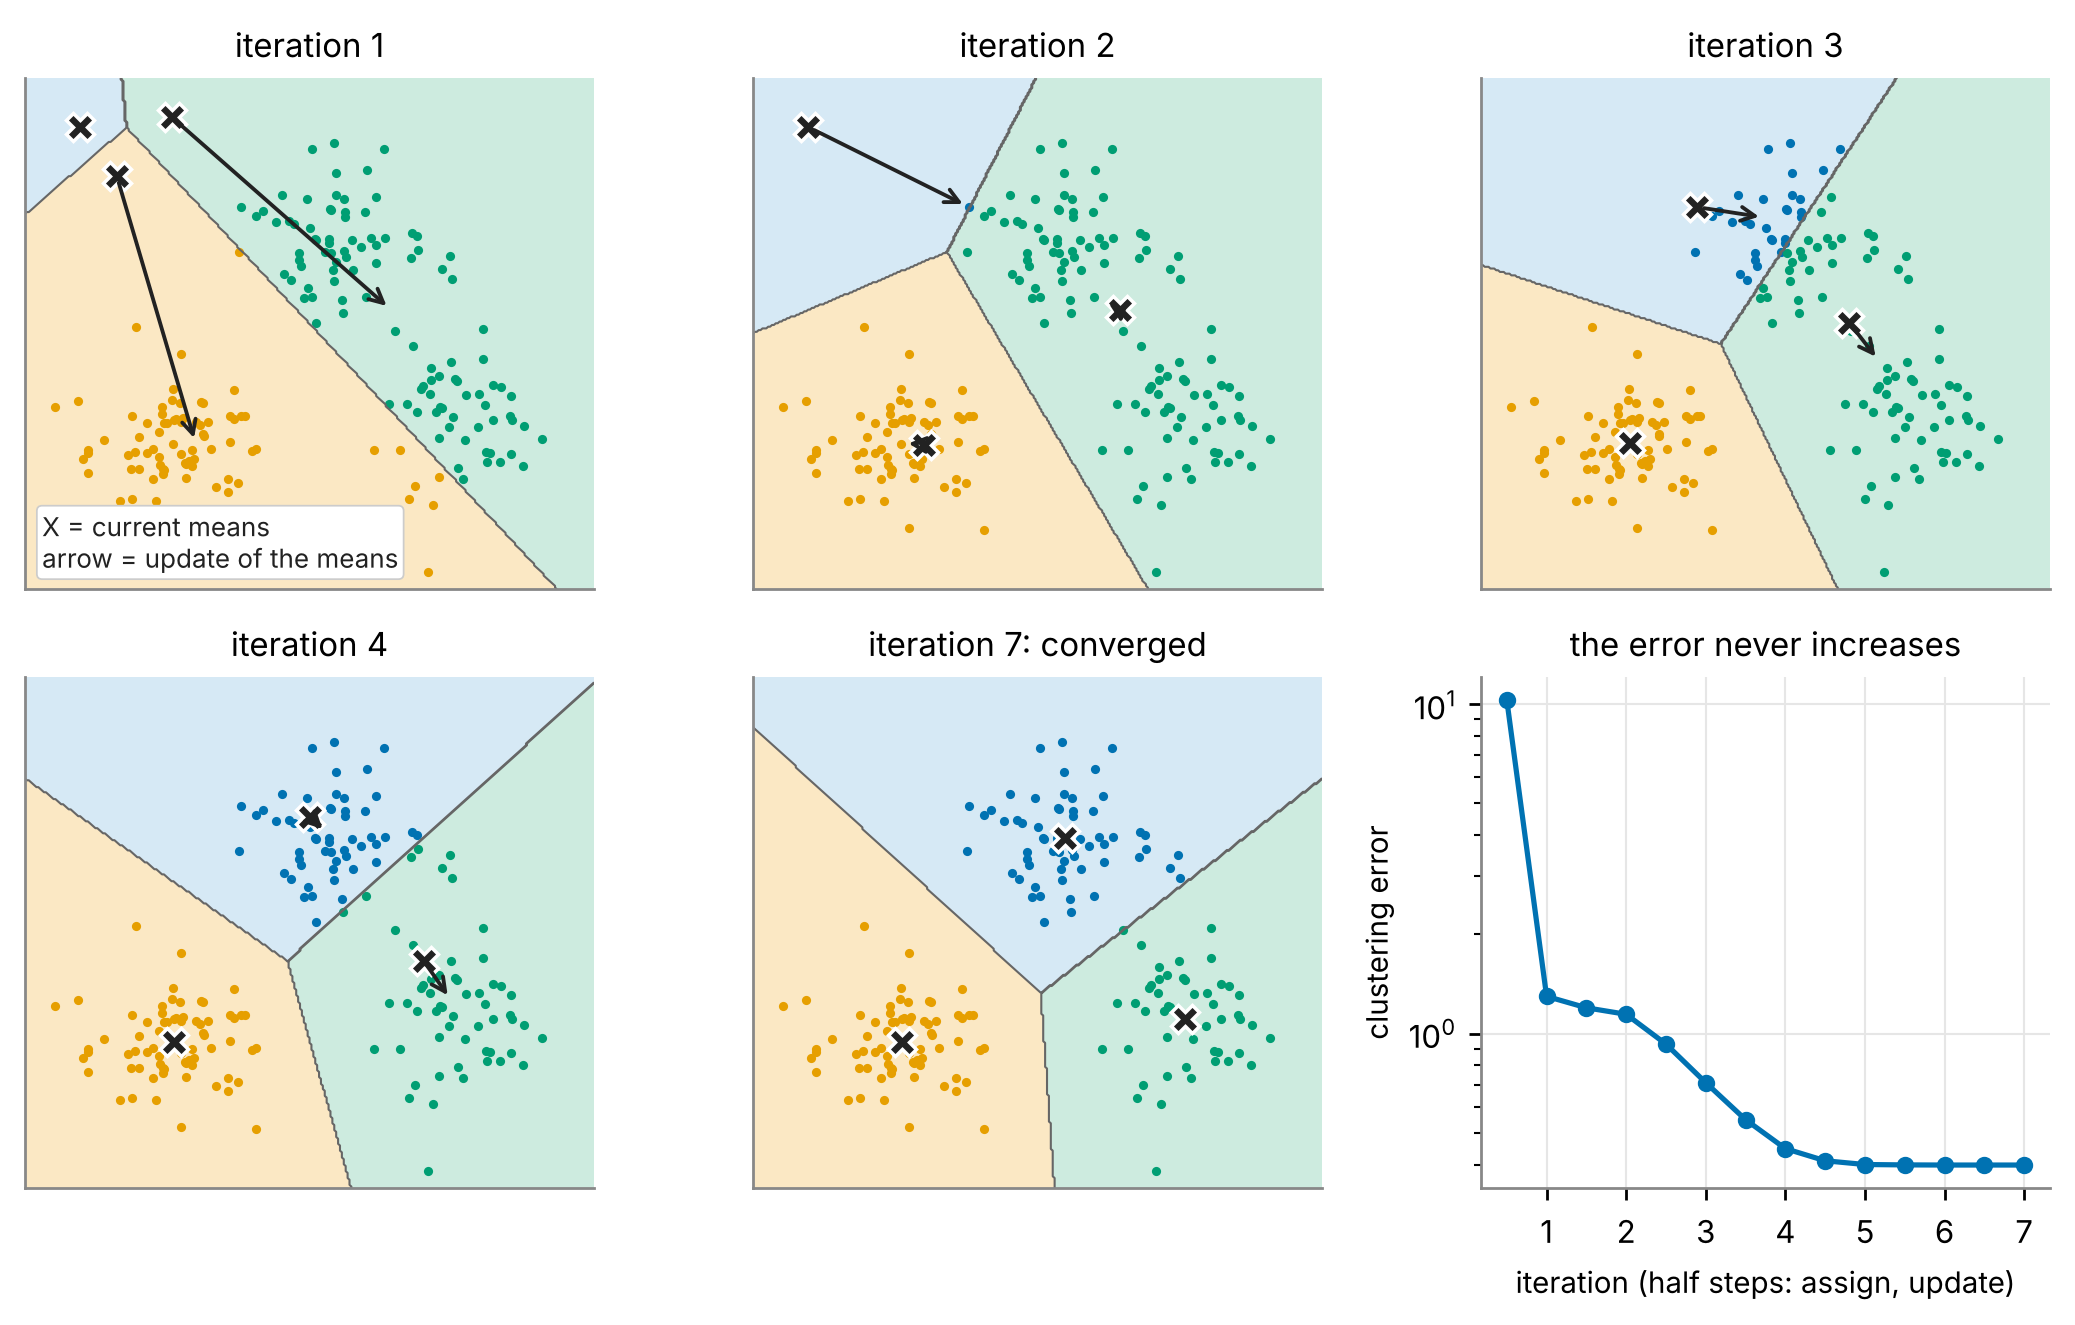
\includegraphics[width=0.8\textwidth]{images/chapter_10/kmeans_iterations.png}
    \caption{k-Means passo per passo: i centri (X) partono male, ma a ogni iterazione si spostano verso i gruppi e l'errore scende.}
\end{figure}

\paragraph*{Esempio del quiz.} Con i dati $10, 7, 7, 5, -1, 10, 2, -3, 0$, $k = 2$ e centri iniziali $10$ e $7$, i centri diventano prima $10$ e $2.43$, poi $8.5$ e $0.6$, poi $7.8$ e $-0.5$, e lì si fermano. L'errore scende da $10.63$ a $5.13$ e poi a $3.53$.

\subsection{GMM: gruppi a ellisse e appartenenze sfumate}
\paragraph*{L'idea.} Ogni gruppo è una nuvola a forma di campana (una gaussiana), che può essere larga o stretta, rotonda o allungata. Invece di dire ``questo punto è del gruppo 2'', il GMM dice ``è al 68\% del gruppo 2 e al 32\% del gruppo 1'' (clustering \emph{soft}).

Conta la distanza misurata rispetto alla larghezza del gruppo. Nell'esempio delle dimensioni dei pacchetti, un flusso da 425 byte è più vicino al gruppo dei pacchetti piccoli, ma quel gruppo è molto stretto, mentre quello dei pacchetti grandi è largo: il GMM gli dà il 68\% di appartenenza al gruppo dei pacchetti grandi. Funziona come k-Means, alternando due passi (stima le appartenenze, aggiorna le gaussiane), e ha gli stessi problemi: serve $k$ e ci si può bloccare in un minimo locale.

\subsection{DBSCAN e clustering gerarchico}
\paragraph*{L'idea.} Quando i gruppi hanno forme strane (curve, anelli) o ci sono punti isolati, centri ed ellissi non bastano più. Si guarda allora chi è collegato a chi.

\textbf{DBSCAN} funziona come il passaparola: un punto con abbastanza vicini (almeno minPts entro un raggio $\varepsilon$) è un punto ``core'', e i punti core vicini tra loro formano un gruppo, qualunque forma abbia. I punti vicini a un core sono di ``bordo''; quelli isolati sono \textbf{rumore}, cioè anomalie. Trova $k$ da solo, ma bisogna scegliere $\varepsilon$ e minPts.

Il \textbf{clustering gerarchico} parte con ogni punto da solo e unisce, una coppia alla volta, i due gruppi più vicini. Il risultato è un albero genealogico dei gruppi, il dendrogramma: tagliandolo a un'altezza diversa si ottiene un numero diverso di gruppi.

\begin{figure}[h]
    \centering
    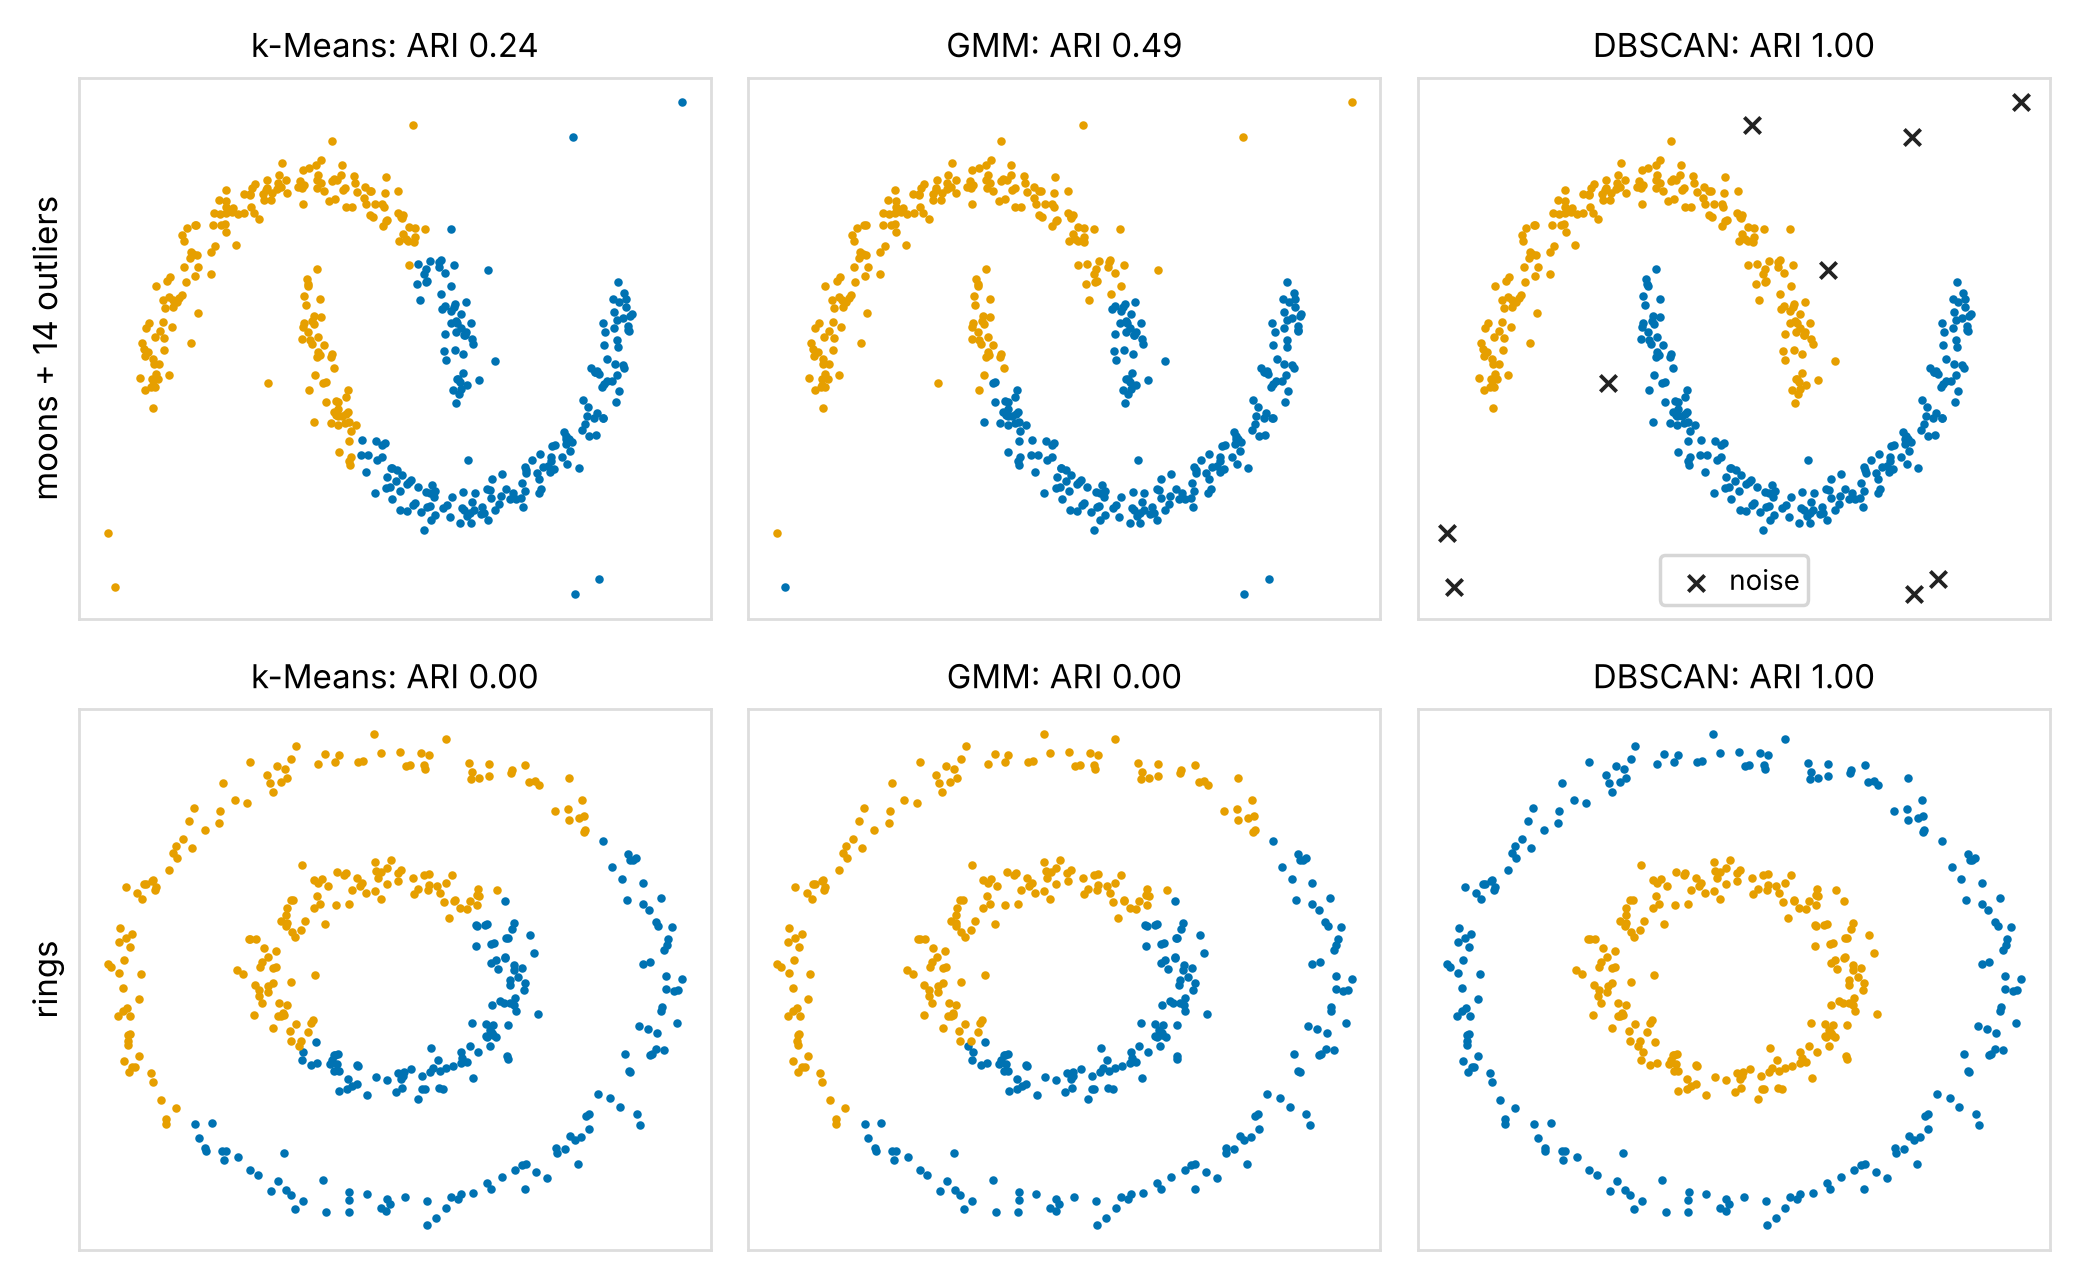
\includegraphics[width=0.8\textwidth]{images/chapter_10/failure_cases.png}
    \caption{Con forme curve e anelli k-Means e GMM sbagliano, DBSCAN segue la forma dei gruppi e marca come rumore i punti isolati.}
\end{figure}

\subsection{Come si giudica un clustering}
\paragraph*{L'idea.} Senza etichette si guarda se i gruppi sono compatti e ben separati (silhouette). Se invece le etichette vere ci sono, per esempio per mettere alla prova il metodo, si confrontano i gruppi con le classi vere (Rand index).

La \textbf{silhouette} di un punto confronta $a$, la distanza media dal suo gruppo, con $b$, la distanza media dal gruppo più vicino: $s = (b-a)/\max(a,b)$. Vicino a $1$ vuol dire ``sta proprio bene dov'è'', vicino a $0$ ``è a cavallo tra due gruppi'', negativo ``è nel gruppo sbagliato''. Esempio: $a = 2$ e $b = 5$ danno $s = 0.6$.

Il \textbf{Rand index} guarda le coppie di punti e conta su quante coppie le due suddivisioni sono d'accordo: insieme in entrambe, oppure separate in entrambe. Nel quiz sono d'accordo $22$ coppie su $36$, quindi $RI = 0.61$. Attenzione: anche suddivisioni del tutto casuali danno un RI intorno a $0.6$. Per questo esiste l'\textbf{adjusted Rand index}, che vale circa 0 per il caso e 1 per l'accordo perfetto; nel quiz è solo $0.24$.

\subsection{Quando usare cosa}
\begin{center}
    \begin{tabular}{l|l}
        \textbf{Situazione} & \textbf{Metodo} \\ \hline
        Gruppi compatti e rotondi, tanti dati     & k-Means \\
        Gruppi allungati o appartenenze incerte   & GMM \\
        Forme strane, outlier da trovare          & DBSCAN \\
        $k$ ignoto, serve la struttura a livelli  & clustering gerarchico \\
        Valutare senza etichette                  & silhouette \\
        Confrontare con classi note               & ARI (meglio del Rand index) \\
    \end{tabular}
\end{center}

\subsection{Da sapere per l'esame}
\begin{center}
    \begin{tabular}{l|l}
        \textbf{Concetto} & \textbf{In una riga} \\ \hline
        Hard e soft       & un gruppo per punto, oppure un grado per ogni gruppo \\ \hline
        Clustering error  & distanza media al quadrato punto--media del gruppo \\ \hline
        k-Means           & assegna al centro più vicino, ricalcola le medie, ripeti \\ \hline
        Proprietà         & l'errore non aumenta mai; si ferma in un minimo locale \\ \hline
        Inizializzazione  & più partenze casuali, si tiene l'errore più basso \\ \hline
        Scelta di $k$     & applicazione, compressione, gomito, silhouette \\ \hline
        GMM               & una gaussiana per gruppo, gradi di appartenenza, EM \\ \hline
        DBSCAN            & punti core, bordo e rumore; trova $k$ da solo \\ \hline
        Gerarchico        & dendrogramma, da tagliare al numero di gruppi voluto \\ \hline
        Silhouette        & $s = (b-a)/\max(a,b)$, da $-1$ a $+1$ \\ \hline
        Rand index        & $(a+b)/\binom{m}{2}$: coppie su cui le partizioni concordano \\ \hline
        ARI               & Rand index corretto per il caso: circa 0 se casuale \\
    \end{tabular}
\end{center}
